\chapter{Revenus et dépenses d'emploi}
\section{Introduction et objectifs}
\subsection{Introduction}
Nous allons voir la nature des revenus d'emploi, comment les employeurs doivent déclarer ces revenus à leurs employés et comment ces derniers doivent les inscrire sur leurs déclarations de revenus.


\subsection{Objectifs}
\begin{itemize}
	\item Expliquer le concept de résidence aux fins de l'impôt du Québec; 
	\item Identifier les étapes à suivre pour préparer les déclarations de revenus;
	\item Compléter la partie \og Identification\fg{} des déclarations de revenus fédérale et provinciale (Québec) des particuliers;
	\item Traiter correctement les types de revenus d'emploi qui sont reportés sur les feuillets de renseignements T4 et relevé~1 (salaires, traitements, allocations imposables, avantages imposables, etc.);
	\item Déclarer les revenus d'emploi qui ne sont pas reportés sur les feuillets de renseignements T4 et relevé~1;
	\item Déterminer le montant des prestations d'assurance salaire ou d'assurance collective contre la maladie ou les accidents qui doit être inclus dans le revenu d'emploi;
	\item Déterminer le montant des subventions de recherche qui doit être inclus dans le revenu d'emploi;
	\item Traiter les paiements versés dans le cadre du Programme de protection des salariés;
	\item Préparer les déclarations T1 et TP-1 jusqu'au revenu total (lignes~15000 de la T1 et 199 de la TP-1, respectivement) pour un particulier qui a un ou des revenus d'emploi seulement.
\end{itemize}


\subsection{Sujets du chapitre}
\begin{itemize}
	\item Réviser l'impôt sur le revenu;
	\item Identification et autres informations;
	\item Régime d'assurance collective;
	\item Calcul du revenu net;
	\item Revenu imposable;
	\item Calcul du revenu total.
\end{itemize}



\section{Étape 1 - \og Identification et autres renseignements\fg{} de la T1}
\begin{intro}
	Qu'elle soit préparée manuellement ou par ordinateur, la déclaration de revenu doit être remplie de manière ordonnée afin de s'assurer que tous les revenus sont déclarés et que toutes les déductions et tous les crédits applicables sont demandés.
\end{intro}


\subsection{Identification}
\begin{itemize}
	\item Nom et adresse postale
	\item Numéro d'assurance sociale
	\item Date de naissance
	\item État civil
	\item Langue de correspondance
\end{itemize}
\arcg{7}

\subsubsection{Nom et prénom}
Si le contribuable a changé de nom au cours de l'année précédente, utilisez le nom actuel.

\subsubsection{Adresse postale}
Le bureau de poste ne transmet pas un chèque de remboursement, mais le renvoie à l'ARC ou Revenu Québec.

\subsubsection{Adresse courriel}
Le champ de courriel doit être laissé vide à moins que le contribuable souhaite s'inscrire pour recevoir des avis par courriel. Pour des raisons de sécurité, les notifications par courriel ne contiennent aucun lien.
\paragraph{Méfiez-vous des escroqueries par hameçonnage possibles}

Ne jamais cliquer sur les liens des courriels.

\cat\href{https://www.canada.ca/fr/agence-revenu/nouvelles/salle-presse/conseils-fiscaux/conseils-fiscaux-2021/comment-savoir-si-lagence-a-communique-avec-vous-et-que-faire-si-cest-le-cas.html}{Comment savoir si l'Agence a communiqué avec vous et que faire si c'est le cas}

\cat\href{https://antifraudcentre-centreantifraude.ca/}{Centre antifraude du Canada}

\subsubsection{\acrfull{nas}}
Premier chiffre:
\begin{description}
	\item[$\boldsymbol{1 \rightarrow 7}$] Résidents canadiens
	\item[9] Résidents temporaires
\end{description}

\subsubsection{Date de naissance}
Particulièrement important:
\begin{itemize}
	\item 65+;
	\item vient d'avoir 18 ou 65~ans.
\end{itemize}

\subsubsection{État civil}
\index{Conjoint}
\begin{description}
	\item[Séparé] A vécu séparément pendant au moins 90 jours
	\item[Conjoint de fait] Après 12 mois de cohabitation
\end{description}

\subsubsection{Informations sur la résidence}
Si le contribuable était un travailleur autonome au cours de l'année d'imposition, inscrivez le nom de la province ou du territoire où l'entreprise était située à la troisième ligne, même s'il s'agit des mêmes renseignements que ceux fournis précédemment. L'impôt provincial sur le revenu d'entreprise est versé à cette province ou à ce territoire, même si le particulier réside dans une autre province. Si l'entreprise du contribuable était située dans plus d'une province ou d'un territoire, tous les emplacements doivent être indiqués, car les impôts devront être répartis.

\subsubsection{Renseignements sur l'époux(se) ou le conjoint(e) de fait}
\index{Conjoint}
\ca
L'ARC utilise le mot \og conjoint\fg{} pour désigner une personne légalement mariée et l'expression \og conjoint de fait\fg{} pour désigner une personne vivant en union de fait. 



\section{Remplir les parties \og Renseignements sur vous\fg{} et  \og Renseignements sur votre conjoint au 31~décembre\fg{} de la TP-1}
\begin{intro}
	Les mêmes informations dans la partie correspondante de la T1 doivent être inscrites dans la partie identification de la TP-1.
\end{intro}


\subsection{Renseignements sur vous}
Revenu Québec n'exige pas du contribuable qu'il qualifie son état civil. Le terme "conjoint ou conjointe" est utilisé pour les couples mariés et en union de fait.
\rqg[s]{15-19}



\section{Exercice 1}
\setcounter{question}{0}
\begin{question}
	Charlotte Landry habite au 1275 rue Giguère, Québec, QC, G1P 1Z6 toute l’année. Son NAS est le 805 101 813 et sa date de naissance est le 5 février 1981. Elle est mariée à Gerald Landry, dont le NAS est le 805 101 821 et la date de naissance est le 15 juillet 1982, et son revenu total en 2023 était de \numprint{22480} \$. Charlotte et Gerald ne sont pas des travailleurs autonomes. Les Landrys n’ont pas d’enfants.
	
	L’adresse courriel de Charlotte est clandry@videotron.ca et elle consent à recevoir de la correspondance en français par voie électronique uniquement.
	
	Complétez les pages 1 des feuillets T1 et TP-1 de Charlotte Landry.
\end{question}
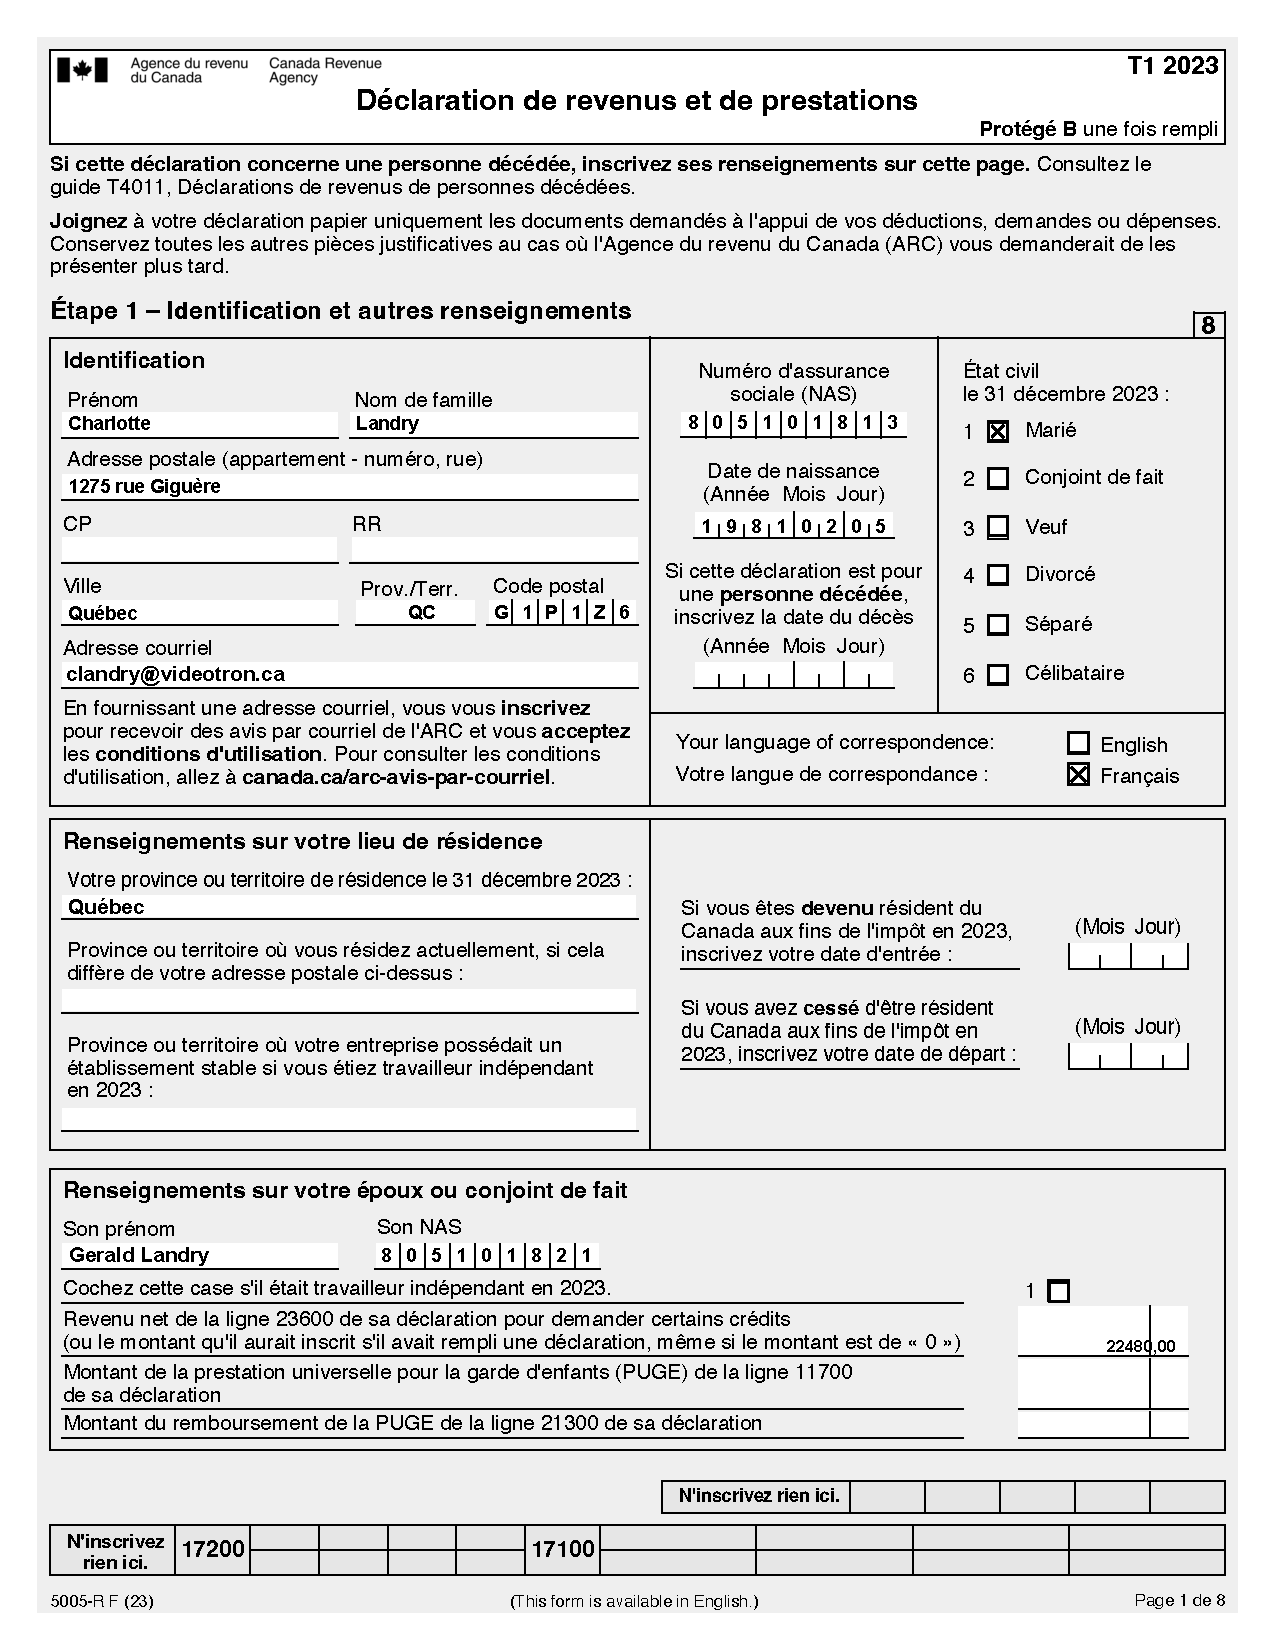
\includepdf[pages={1}, scale=.67, pagecommand={}]{exercice/2-1/Q1/5005-R-2023f-1.pdf}
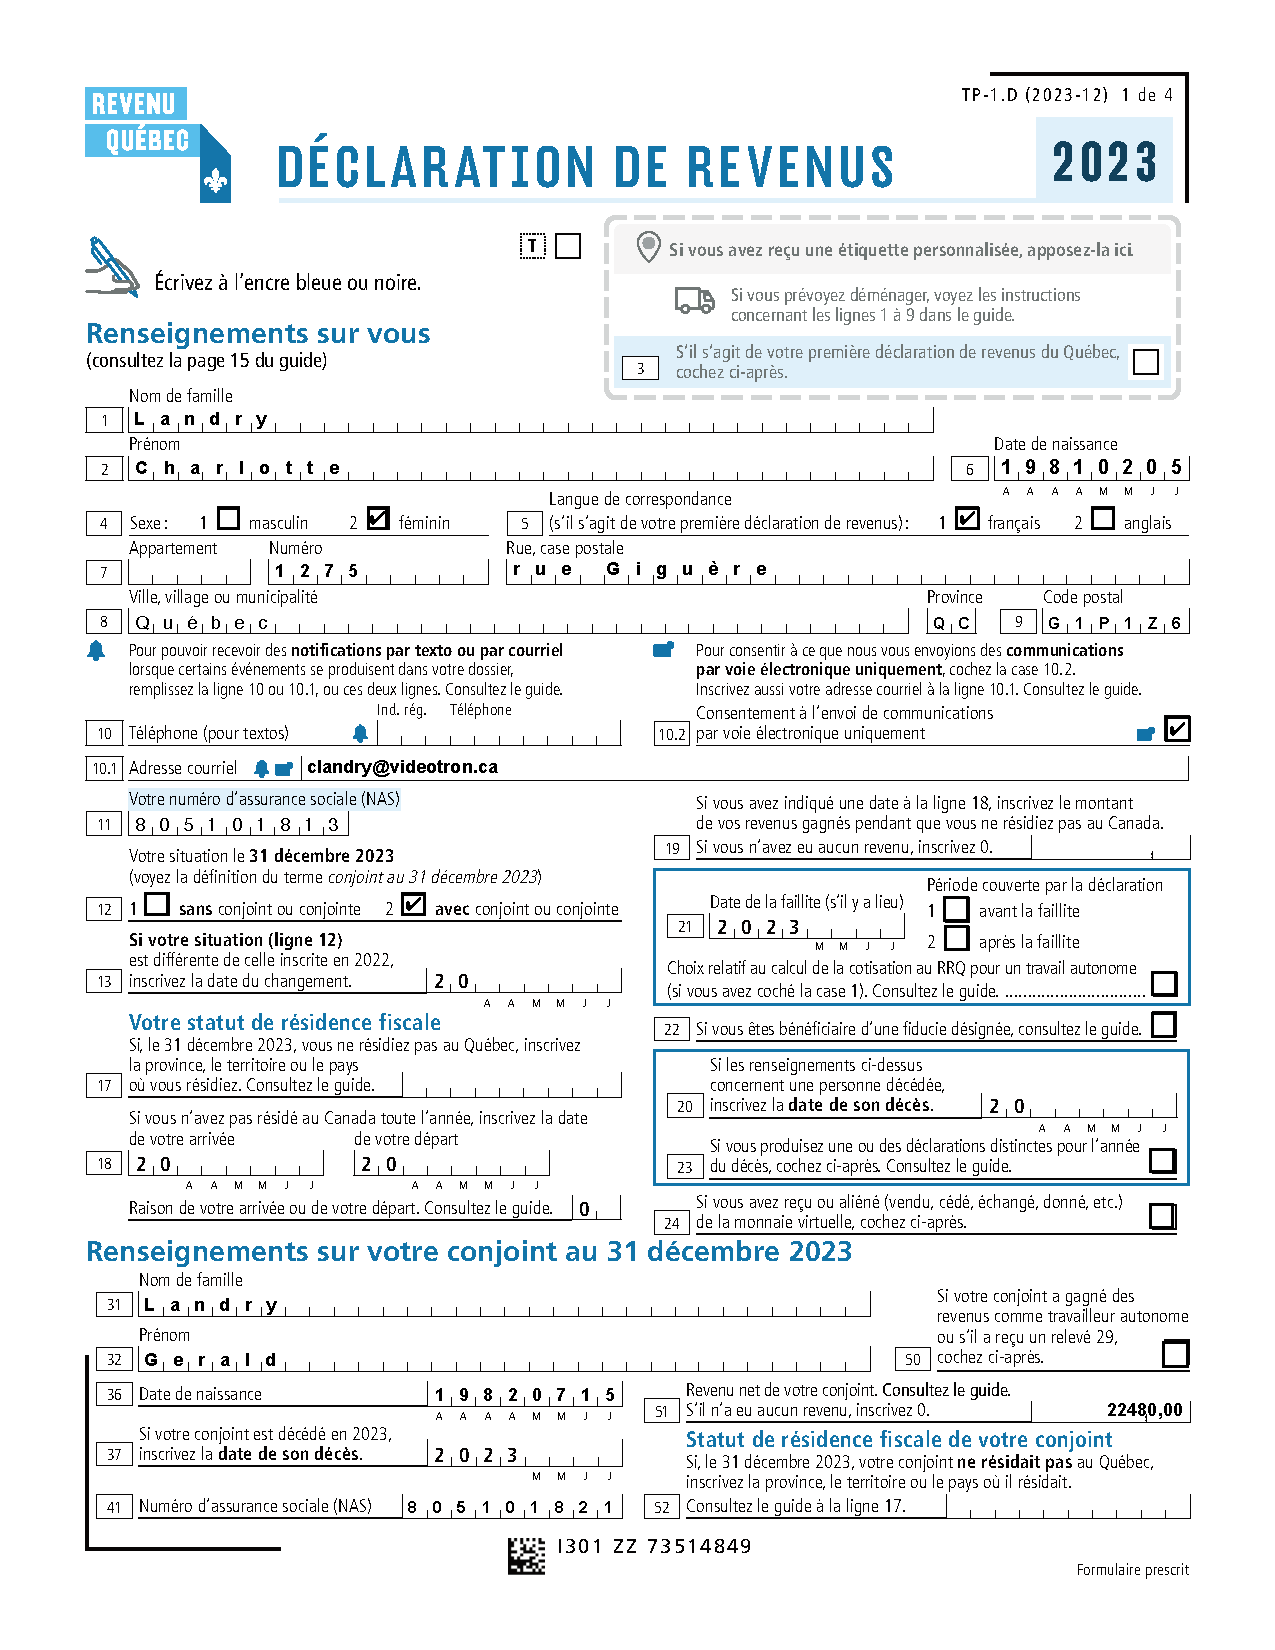
\includepdf[pages={1}, scale=.67, pagecommand={}]{exercice/2-1/Q1/TP-1.D(2023-12)-1.pdf}

\begin{question}
	Le NAS d’Amanda Smith est le 805 101 839. Elle habite au 12 Golf View Crescent dans Montréal, Québec, H3C 3N3. Elle est née le 19 février 1947 et est veuve depuis plusieurs années. Elle n’est pas travailleuse autonome et n’a pas d’adresse courriel. Son numéro de téléphone est le (514) 777-1234.
	
	Complétez la page 1 du livre d’Amanda déclarations de revenus.
\end{question}
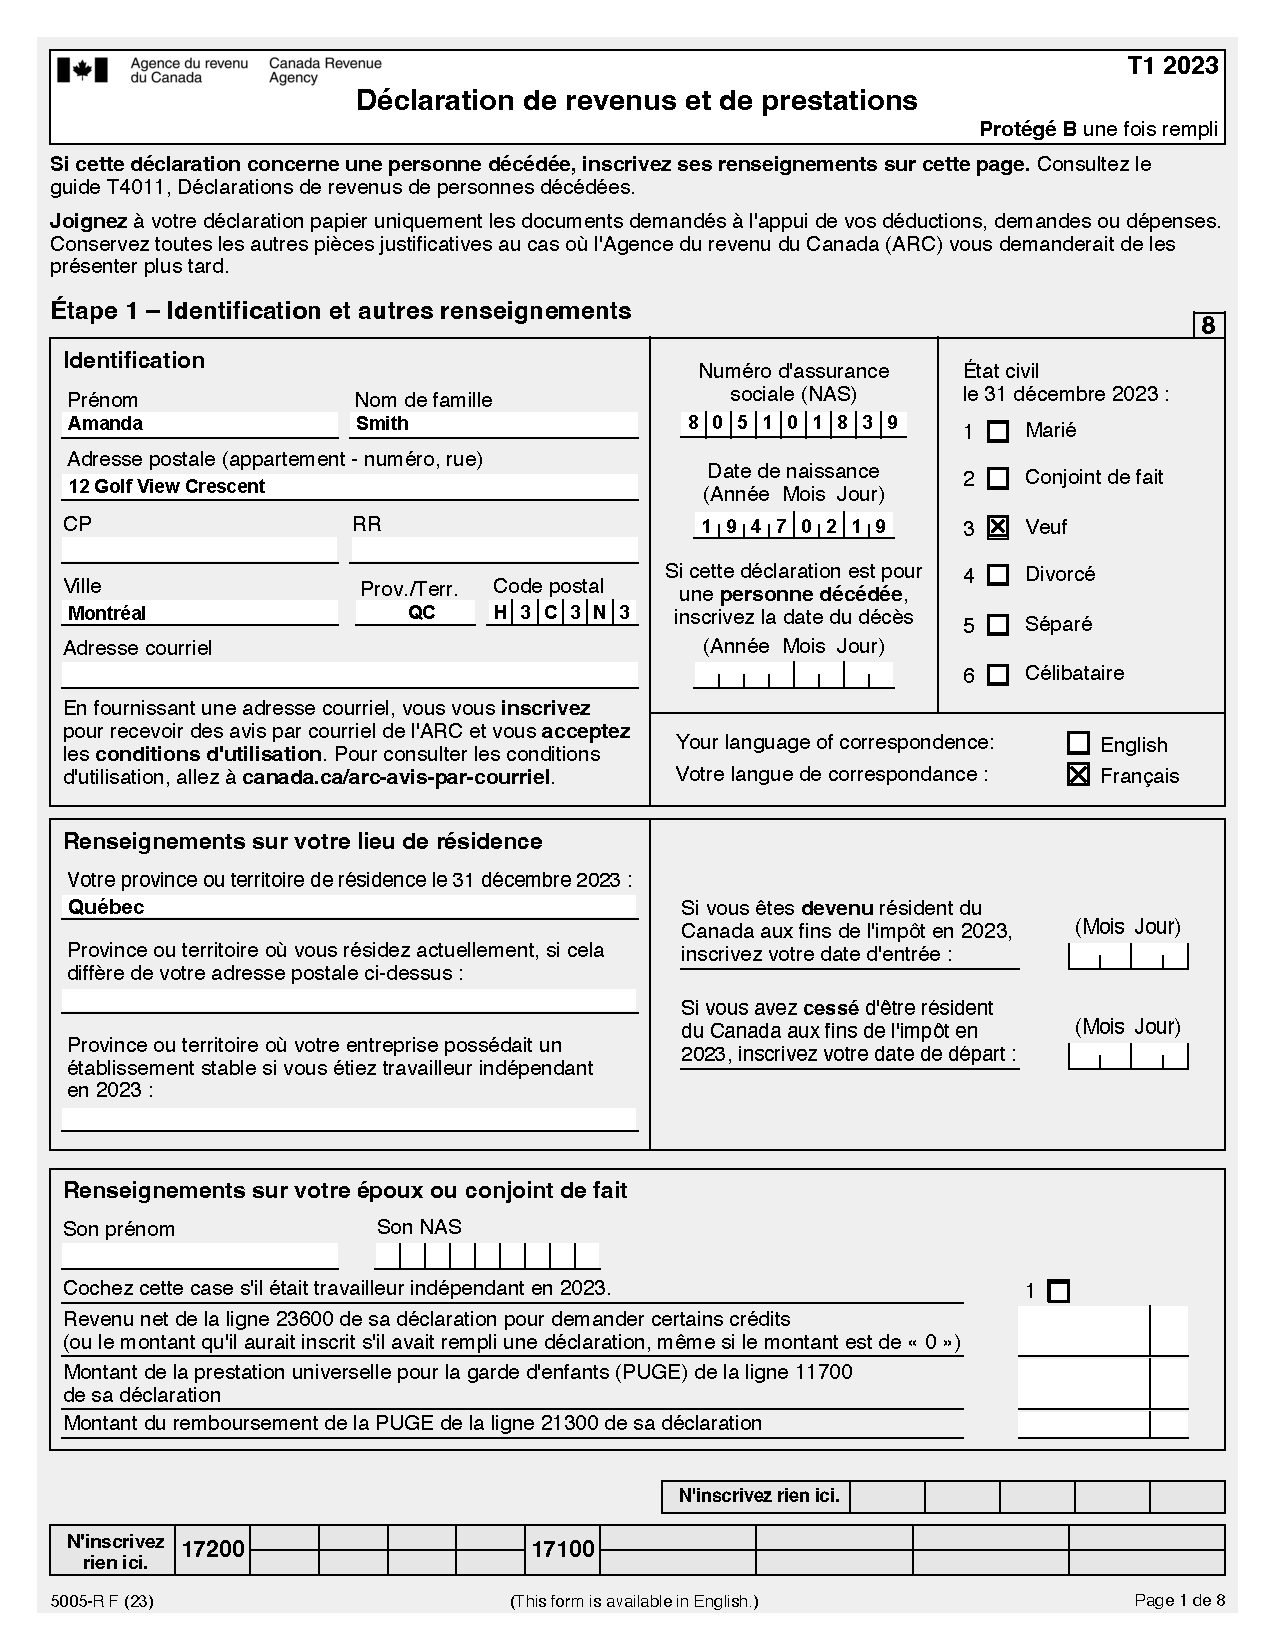
\includepdf[pages={1}, scale=.67, pagecommand={}]{exercice/2-1/Q2/5005-R-2023f-1.pdf}
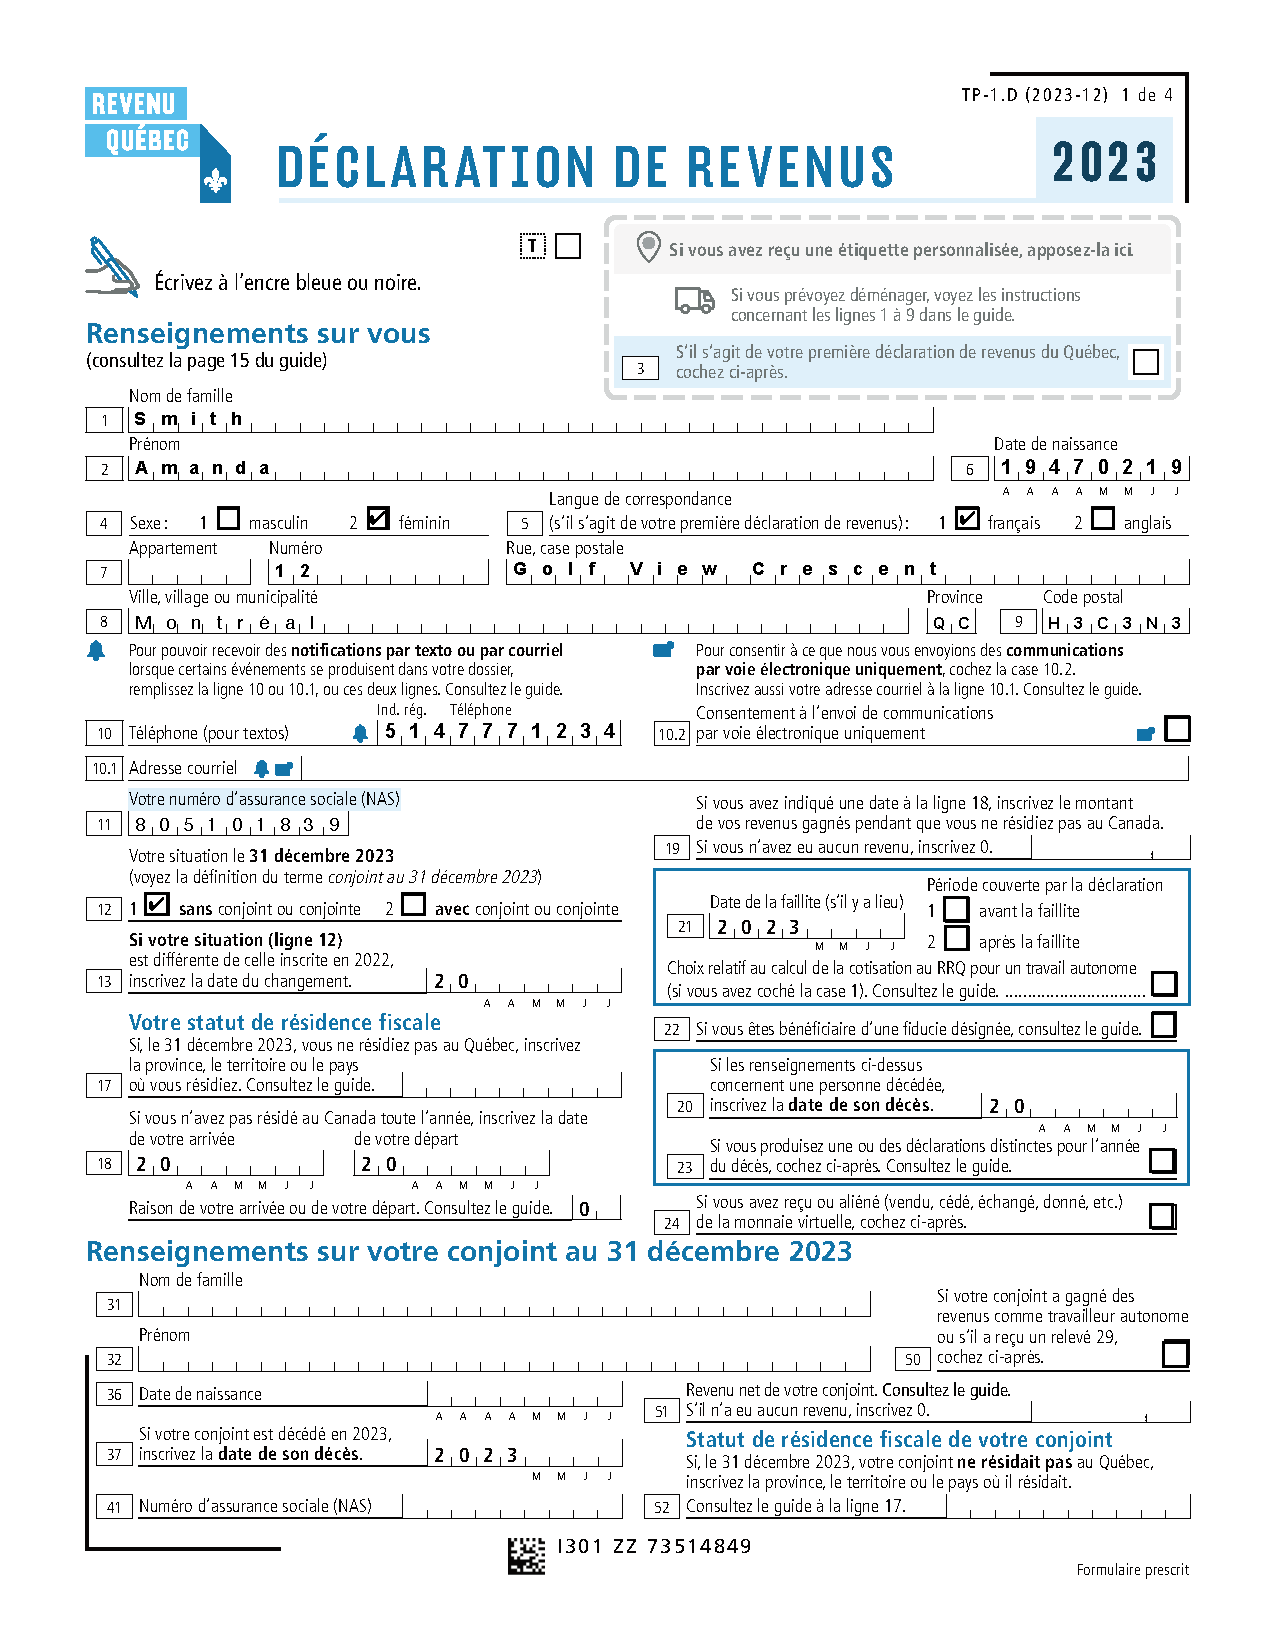
\includepdf[pages={1}, scale=.67, pagecommand={}]{exercice/2-1/Q2/TP-1.D(2023-12)-1.pdf}



\section{Élections Canada}
\begin{intro}
	Élections Canada tient à jour une base de données automatisée appelée le Registre national des électeurs. La liste est mise à jour à l'aide des renseignements fournis par les organismes gouvernementaux, y compris l'ARC. Le registre est également utilisé pour créer des listes pour les élections provinciales, municipales et scolaires.
\end{intro}
À quelques exceptions près, il est interdit à l'ARC de communiquer des renseignements sur les contribuables sans le consentement de ceux-ci.


\subsection{Comment répondre à la question B)}
Répondre \og Oui\fg{} autorise l'ARC à fournir le nom, l'adresse, la date de naissance et le statut de citoyenneté canadienne à Élections Canada
\arcg{9}



\section{Exercice 2}
\setcounter{question}{0}
\begin{question}
	Si vous êtes citoyen canadien et que vous répondez \og Oui\fg{} à la question d'Élections Canada, votre nom sera-t-ilajouté à la liste Registre des électeurs?
\end{question}
Oui, si vous êtes un électeur éligible.

\begin{question}
	Quelles sont les conséquences d'une réponse \og non\fg{} à la question Élections Canada?
\end{question}
Répondre \og Non\fg{} signifie que les renseignements personnels d'un contribuable ne sont pas mis à jour. Par conséquent, les contribuables qui déménagent ont la responsabilité d'aviser Élections Canada afin que leur nom apparaisse sur la bonne liste électorale. Le fait de répondre \og Non\fg{} ne supprime pas le nom d'un contribuable de la liste.



\section{Loi sur les Indiens - Revenu exonéré}
\begin{intro}
	L'ARC a le formulaire \href{https://www.canada.ca/fr/agence-revenu/services/formulaires-publications/formulaires/t90.html}{T90 Revenu exonéré d'impôt selon la Loi sur les Indiens}, qui doit être rempli.
\end{intro}

\begin{note}
	L'ARC a besoin de ces informations pour déterminer correctement le crédit canadien pour la formation et pour déterminer si le contribuable a droit à l'\acrfull{act}, qui est traitée au chapitre~7.
\end{note}



\section{Les biens étrangers}
\ca
\begin{intro}
	Les résidents canadiens doivent déclarer leurs revenus de toutes sources, que ce soit au Canada ou à l'étranger. Afin de s'assurer que tous les revenus étrangers sont déclarés, tous les contribuables, à l'exception de ceux qui ont immigré au Canada au cours de l'année, doivent répondre à la question. Il n'y a aucune partie correspondante sur la TP-1.
\end{intro}
Si le contribuable répond \og Oui\fg{}, il doit remplir le formulaire T1135


\subsection{Formulaire T1135 - Bilan de vérification du revenu étranger}
\cat\href{https://www.canada.ca/fr/agence-revenu/services/formulaires-publications/formulaires/t1135.html}{T1135 Bilan de vérification du revenu étranger}

\subsubsection{Biens qui doivent être déclarés}
Le contribuable doit produire le T1135 si le coût total de tous les biens détenus au cours de l'année d'imposition, et non sa valeur actuelle, dépasse \numprint{100000}~\$.

Si un contribuable hérite d'un bien, le coût d'acquisition correspond à la juste valeur marchande (JVM) à la date de l'héritage. Pour un immigrant venant au Canada, le coût de ses biens étrangers sera considéré comme la JVM à la date d'immigration.

Biens qui doivent être déclarés:
\begin{itemize}
	\item Les comptes bancaires étrangers;
	\item Les fonds de terre et les biens locatifs hors du Canada;
	\item Les actions dans des sociétés étrangères;
	\item Les unités dans des fonds communs de placement établis sur un territoire étranger.
\end{itemize}

Les fonds communs de placement établis au Canada qui font des investissements à l'étranger sont exclus.

\begin{note}
	Les biens étrangers comprennent aussi les biens qui ne génèrent aucun revenu (par exemple, un terrain vacant).
\end{note}

\subsubsection{Biens qui ne doivent pas être déclarés}
\begin{itemize}
	\item Les biens à usage personnel;
	\item Les biens utilisés ou détenus exclusivement dans le cadre d'activités d'une entreprise exploitée activement;
	\item Une participation dans un \og Individual retirement account (IRA)\fg{} aux États-Unis (équivalent américain du régime enregistré d'épargne-retraite canadien);
	\item Les biens étrangers détenus dans un REER ou un compte d'épargne libre d'impôt (CELI) n'ont pas à être déclarés.
	\item Les pensions étrangères ou régimes de retraite qui sont exempts d'impôts dans le pays étranger;
	\item Une participation dans une fiducie étrangère pour laquelle ni le contribuable ni quelqu'un qui lui est lié, n'a dû payer (par exemple, une succession).
\end{itemize}

Un bien à usage personnel est un bien utilisé principalement à des fins d'agrément personnel, comme un véhicule, une propriété de vacances, des bijoux, des œuvres d'art et tout autre bien semblable. Si un bien immobilier est utilisé comme une propriété de vacances pour une partie de l'année et est loué pour le restant de l'année, il doit être déclaré sur le formulaire T1135 si le contribuable loue le bien avec un espoir raisonnable de profit. Cependant, s'il n'y a aucune attente raisonnable de profit et que la personne récupère simplement une partie des dépenses, le bien est exclu de l'obligation de déclaration.

\begin{note}
	Si le contribuable choisit d'utiliser la partie B pour décrire les biens étrangers en sa possession, il doit utiliser la partie B pour tous ses biens étrangers déterminés.
\end{note}

Les contribuables qui, à un moment donné de l'année, possédaient des biens étrangers déterminés d'un coût de \numprint{250000}~\$    ou plus, doivent utiliser la méthode détaillée, partie B.

\begin{note}
	Lorsque vous remplissez le formulaire T1135 pour un particulier, il est nécessaire de choisir le code de personne approprié:
	\begin{enumerate}
		\item Le particulier ou son époux (conjoint de fait) est un travailleur autonome.
		\item Le particulier et son époux (conjoint de fait) ne sont pas des travailleurs autonomes.
	\end{enumerate}
\end{note}


\subsection{Méthode de déclaration simplifiée}
Si le coût total est inférieur à \numprint{250000}~\$, il est possible de faire une déclaration simplifiée.


\subsection{Rapports agrégés}
Les contribuables qui détiennent des biens étrangers dans un compte auprès d'un courtier en valeurs mobilières inscrit au Canada ou d'une société Canadian Trust sont autorisés à déclarer la juste valeur marchande combinée de tous ces biens pays par pays à la fin de l'année d'imposition au lieu de déclarer les détails de chaque bien. Les biens étrangers déterminés ne comprennent pas les biens détenus dans un régime enregistré et les fonds communs de placement enregistrés au Canada.

\subsubsection{Les contribuables qui choisissent cette option doivent déclarer leurs biens à la section~7 de la partie B du formulaire T1135:}
\begin{itemize}
	\item Tous les biens détenus auprès d'un courtier en valeurs mobilières inscrit au Canada ou d'une société Canadian Trust en particulier doivent être regroupés pays par pays.
	\item Au lieu de fournir le montant du coût des biens, les contribuables doivent fournir leur juste valeur marchande à la fin de l'année et la juste valeur marchande maximale des biens au cours de l'année (qui peut être fondée sur leur juste valeur marchande maximale à la fin du mois).
\end{itemize}

Il y a une pénalité de 25 \$ par jour pour chaque jour où le formulaire T1135 n'est pas produit, jusqu'à concurrence de 2 500 \$.



\section{Exercice 3}
\setcounter{question}{0}
\begin{question}
	Quel est le but de la question à l'égard des biens étrangers?
\end{question}
Le gouvernement fédéral utilise ces renseignements pour vérifier si le contribuable a déclaré tous les revenus qu'il a reçus ou pourraient recevoir de sources étrangères.

\begin{question}
	Quelle est la pénalité pour défaut de produire un formulaire T1135 à l'heure?
\end{question}
25~\$ par jour pour chaque jour de retard, avec un maximum de
\numprint{2500}~\$.

\begin{question}
	Au cours de l'année d'imposition, un résident canadien a acheté un terrain vacant aux États-Unis au prix de \numprint{135000}~\$ CA. Comme le terrain ne produit pas de revenu, le contribuable n'est pas tenu de le déclarer sur un T1135.
	
	L'énoncé ci-dessus est-il vrai ou faux? Expliquez votre réponse.
\end{question}
FAUX. Les biens étrangers qui doivent être déclarés comprennent les biens qui ne génèrent aucun revenu, comme un terrain vacant.

\begin{question}
	Bill a des actions étrangères dans une société américaine, ABC Inc., qui coûtait \numprint{120000}~\$ CAN il y a dix ans. Ces actions valaient \numprint{80000}~\$ en 2023. Devez-vous produire un formulaire T1135 pour 2023? Expliquer.
\end{question}
Oui, parce que le coût est supérieur à 100 000 dollars. La valeur n'a pas d'importance.

\begin{question}
	Larry a trois investissements étrangers: un compte bancaire de \numprint{40000}~\$CAN, actions d'une société britannique qui ont coûté \numprint{50000}~\$CAN et un immeuble locatif français qui a coûté \numprint{60000}~\$CAN. Larry doit-il produire le formulaire T1135? Expliquez.
\end{question}
Oui, car le coût total de tous les biens étrangers s'élève à 150 000 dollars, ce qui est supérieur à \numprint{100000}~dollars.

\begin{question}
	Irania a acheté une propriété locative américaine qui coûtait \numprint{75000}~\$ il y a cinq ans. En 2023, ce valait \numprint{130000}\$CAN. Doit-elle produire le formulaire T1135 pour 2023? Expliquez.
\end{question}
Non, parce que le coût total est inférieur à \numprint{100000}~dollars. La valeur n'a pas d'importance.

\begin{question}
	Bob a acheté une maison de vacances aux États-Unis pour \numprint{150000}~\$ CAN. Seuls Bob et sa famille utilisent cette propriété et il ne loue pas. Bob doit-il produire le formulaire T1135? Expliquez.
\end{question}
Non, parce que cette maison de vacances est utilisée uniquement comme bien à usage personnel, le formulaire T1135 ne doit pas être rempli.



\section{Revenu d'emploi}
\begin{intro}
	Explication de ce qu'est un revenu d'emploi et comment les feuillets de renseignements T4 et Relevé1 remis au contribuable sont utilisés pour contribuer au calcul du revenu total.
\end{intro}
Les revenus d'emploi impliquent une relation d'employeur-employé(e). Ils comprennent également les revenus provenant d'une charge.

\begin{description}
	\index{Charge}
	\item[Charge] Poste occupé par un particulier, qui donne droit à une rémunération. Cette fonction peut être un poste de juge, de député, de directeur d'une société publique, de conseiller municipal ou de commissaire d'école.
	\index{Rémunération}
	\item[Rémunération] Salaire et toute autre somme d'argent versé par un particulier en tant qu'employeur ou en tant que payeur.
\end{description}


\subsection{Employé ou travailleur autonome?}
Pour déterminer si un contribuable est un employé ou un travailleur autonome, il faut considérer le degré de contrôle qui existe entre les différentes parties.

Pour les employées et les employés, le travail qu'ils doivent accomplir est contrôlé par l'employeur. Celui-ci décide la manière dont le travail est effectué et de l'horaire de l'employé.  

Par contre, un travailleur autonome est libre de choisir les produits ou services qu'il va offrir, les clients qu'il va rencontrer, les heures pendant lesquelles il va travailler, le prix qu'il va demander pour ses produits ou services, et il peut engager du personnel pour faire le travail.
\begin{note}
	Il est tout à fait normal qu'un travailleur indépendant soit à la fois indépendant et salarié. Cependant, il est toujours considéré et traité comme un travailleur indépendant.
\end{note}



\section{Exercice 4}
\setcounter{question}{0}
\begin{question}
	Les revenus d'emploi comprennent notamment les revenus provenant d'une charge. Donnez trois exemples d'emplois qui sont considérés comme une charge.
\end{question}
Quelques exemples: juge, membre du Parlement, directeur de société, conseiller municipal, directeur d'une entreprise publique.

\begin{question}
	Aline travaille comme gardienne d'enfants. Elle prend soin d'un bébé pendant plusieurs heures par jour au domicile des parents. Les parents du bébé déterminent le nombre d'heures qu'Aline doit travailler, ainsi que les tâches qu'elle doit accomplir pendant qu'elle se trouve à leur domicile. 
	
	Aline est-elle une employée ou une travailleuse autonome? Expliquez votre réponse.
\end{question}
Aline est une employée des parents du bébé parce que ces derniers contrôlent le travail qu'elle fait et à quel moment elle doit le faire.

Les parents devraient lui émettre un T4 et un relevé~1 pour le revenu gagné.

\begin{question}
	Gisèle garde des enfants du voisinage à son domicile. Elle décide de ses heures de disponibilité, du tarif qu'elle va demander et des clients qu'elle va accepter. 
	
	Gisèle est-elle une employée ou une travailleuse autonome? 
	Expliquez votre réponse.
\end{question}
Gisèle est une travailleuse autonome, car elle contrôle ses heures de travail, le prix qu'elle demande et elle choisit ses clients.



\section{Déclarer un revenu d'emploi}
\begin{intro}
	Les revenus d'emploi sont déclarés sur plusieurs lignes des formulaires T1 et TP-1, selon le type et la source des revenus. Dans cette section, nous nous concentrerons sur la façon de traiter les revenus déclarés sur un T4 et un Relevé~1 reçu de l'employeur.
\end{intro}
Fédéral:
\ca
\begin{description}
	\item[10100] Revenus d'emploi (T4.14)
	\item[10120] Commissions incluses à la ligne~10100 (T4.42)\footnote{\label{ATitreDInformation}À titre d'information}
	\item[10130] Cotisations à un régime d'assurance-salaire (cf. ligne~\href{https://www.canada.ca/fr/agence-revenu/services/impot/particuliers/sujets/tout-votre-declaration-revenus/declaration-revenus/remplir-declaration-revenus/revenu-personnel/ligne-10100-revenus-emploi.html}{10100})
	\item[10400] Autres revenus d'emploi
	\item[13000] Autres revenus
\end{description}

Québec:
\qc
\begin{description}
	\item[100] Commissions reçues (RL1.M)\textsuperscript{\,\ref{ATitreDInformation}}
	\item[101] Revenus d'emploi (RL1.A)
	\item[105] Correction des revenus d'emploi, si RL22
	\item[107] Autres revenus d'emploi
	\item[154] Autres revenus
\end{description}


\subsection{Feuillets de renseignements}
L'utilisation des feuillets de renseignements facilite grandement la tâche de préparation des déclarations de revenus.


\subsection{Feuillets T4 et relevés 1}
Au fédéral, l'employeur doit remplir un feuillet T4 pour chaque personne pour les raisons suivantes:
\begin{itemize}
	\item Il a versé une rémunération de plus de 500~\$ pendant l'année;
	\item Il a prélevé des cotisations pour le RRQ, pour l'AE et pour le RQAP; ou
	\item Il a prélevé de l'impôt fédéral sur le revenu.
\end{itemize}

\begin{note}
	Nous expliquerons les acronymes RRQ, AE et RQAP plus loin dans cette partie.
\end{note}
\cat\href{https://www.canada.ca/fr/agence-revenu/services/formulaires-publications/formulaires/t4.html}{T4 État de la rémunération payée (feuillet)}

Au Québec, l'employeur doit émettre un relevé~1 pour tous les salaires et les autres sommes qu'il a versés à un employé ou une employée, peu importe le montant versé.

\begin{note}
	Avant d'inscrire les montants du T4 sur la T1, vérifiez l'année et la province d'emploi.
\end{note}
\qct\href{https://www.revenuquebec.ca/fr/services-en-ligne/formulaires-et-publications/details-courant/rl-1/}{Relevé~1 – Revenus d'emploi et revenus divers }


\subsubsection{case~14 du T4 et case~A du relevé~1}
Ces revenus doivent être reportés aux lignes~10100 de la T1 et 101 de la TP-1.

Les montants inscrits aux cases~14 du T4 et A du relevé~1 comprennent, entre
autres:
\begin{itemize}
	\item Les traitements, les salaires, les commissions, les pourboires, les primes, les paies de vacances, les allocations imposables;
	\item La valeur des avantages imposables liés à l'emploi et la compensation versée aux volontaires participant à des services d'urgence.
\end{itemize}

\begin{note}
	Les montants déclarés à la case~14 du T4 et à la case~A du Relevé~1 ne sont pas toujours égaux. Certains avantages, fournis par l'employeur, peuvent être désignés comme imposables par l'ARC et Revenu Québec et, par conséquent, sont inclus à la case~14 et à la case~A.
	
	Cependant, certaines prestations sont considérées comme imposables par le Québec, mais pas par le gouvernement fédéral. L'inverse est également vrai, mais le plus souvent, la case~A sera plus élevée que la case~14.
\end{note}

\subsubsection{Retenues à la source et autres montants inscrits sur les T4 et relevé~1}
Montants retenus à la source:
\begin{itemize}
	\item L'impôt fédéral (case~22 du T4) et l'impôt provincial (case~E du relevé~1);
	\item Les cotisations au Régime des rentes du Québec (cases~17 du T4 et B du relevé~1);
	\item Les cotisations à l'assurance emploi (cases~18 du T4 et C du relevé~1);
	\item Les cotisations au Régime québécois d'assurance parentale (cases~55 du T4 et H du relevé~1);
	\item Les cotisations à un Régime de pension agréé (cases~20 du T4 et D du relevé~1), si l'employeur a un tel régime;
	\item Les cotisations syndicales (cases~44 du T4 et F du relevé~1);
	\item Les dons de bienfaisance (cases~46 du T4 et N du relevé~1).
\end{itemize}

Autres montants:
\begin{itemize}
	\item Les gains assurables à l'assurance emploi (case~24 du T4);
	\item Le salaire admissible au Régime des rentes du Québec (cases~26 du T4 et G du relevé~1);
	\item Le salaire admissible au Régime québécois d'assurance parentale (cases~56 du T4 et I du relevé~1);
	\item Le facteur d'équivalence, s'il y a lieu (case~52 du T4).
\end{itemize}

\index{Gains assurables}
\index{Salaires admissibles}
Le terme \textbf{gains assurables} utilisé dans le T4 signifie la même chose que le terme \textbf{salaires admissibles} utilisé dans le Relevé~1.

\subsubsection{Commissions}
Si le revenu brut d'emploi inscrit aux cases~14 du T4 et A du relevé~1 inclut des commissions, ces dernières sont inscrites séparément aux cases~42 du T4 et M du relevé~1. La case~42 du T4 doit être inscrite par l'employeur au bas du feuillet, dans la partie \og Autres renseignements\fg{}.

Les commissions reçues doivent être reportées aux lignes~10120 de la T1 et 100 de la TP-1. Ces deux lignes sont pour information seulement.
Les commissions sont déjà incluses dans le montant de la case~14 et dans celui de la case~A. On ne doit pas les ajouter à nouveau au montant des lignes~10100 de la T1 et 101 de la TP-1. 

\subsubsection{Allocations et avantages découlant d'un emploi.}
Si un employeur fournit des avantages ou allocations à un employé, il doit toujours déterminer si l'avantage qu'il lui fournit est imposable et doit être inclus dans le revenu d'emploi de l'employé.

\subsubsection{Inscription sur les feuillets de renseignements T4 et relevés 1}
Voici des exemples d'allocations ou d'avantages imposables:
\begin{itemize}
	\item Le logement, la pension et les repas gratuits ou subventionnés (cases~30 du T4 et V du relevé~1);
	\item Les avantages relatifs aux voyages effectués par un résident d'une région éloignée reconnue (cases~32 du T4 et K du relevé~1). La case~33 du T4 existe pour l'aide accordée pour les voyages pour soins médicaux, mais le montant est inclus dans la case~32;
	\item L'allocation pour l'utilisation d'un véhicule à moteur (cases~40 et L);
	\item L'utilisation à des fins personnelles d'une voiture de l'employeur – Automobile mise à la disposition d'un employé (cases~34 et W);
	\item Les prêts sans intérêt ou à faible intérêt, consentis par l'employeur à un employé (cases~36 et L);
	\item Les avantages liés aux options d'achat de titres (cases~38 et L);
	\item Les autres avantages imposables comme les avantages associés aux:
	\begin{itemize}
		\item Primes d'assurance maladie, d'assurance salaire non collectif, d'assurance-vie,
		\item Frais de voyages, frais de scolarité et à d'autres frais, payés par l'employeur au bénéfice de l'employé (cases~40 et L),
		\item Cotisations de l'employeur aux prestations forfaitaires pour un régime d'assurance salaire;
	\end{itemize}
	\item Au Québec seulement, les cotisations versées par l'employeur au bénéfice de l'employé à un régime privé d'assurance maladie (case~J) ou à un régime d'assurance interentreprises (case~P).
\end{itemize}
\begin{note}
	C'est une très bonne pratique que de vérifier l'usage de chaque case à l'aide des informations figurant au verso de chaque feuillet.
	
	Ces avantages imposables sont inscrits distinctement dans d'autres cases à titre d'information seulement, ils sont déjà inclus dans les cases~14 du T4 et A du RL-1. 
	
	Par conséquent, il ne faut pas les ajouter à nouveau dans le revenu, pour éviter d'être imposé une deuxième fois sur le même montant. 
\end{note}

\subsubsection{Avantage relatif à un ancien emploi}
\qc
Si le montant de la case~A comprend uniquement la valeur d'un avantage (en argent ou en nature) que le contribuable reçoit ou dont il bénéficie dans l'année en raison d'un ancien emploi, l'employeur doit remplir une case~Supplémentaire sur le relevé~1. 
Note.

\begin{note}
	Le montant de la case~A devrait être égal à la somme des cases suivantes: J, K, L, P, V et W.
\end{note}
\[ A = J + K + L + P + V + W\]
\begin{description}
	\item[A] Revenus d'emploi
	\item[J] Régime privé d'assurance maladie 
	\item[K] Voyages (région éloignée) 
	\item[L] Autres avantages
	\item[P] Régime d'assurance interentreprises 
	\item[V] Nourriture et logement 
	\item[W] Véhicule à moteur 
\end{description}

La case~Vierge supplémentaire que l'employeur doit remplir est la case~211. Cette case~Sera suivie du montant de la case~A.

La case~211 est d'une grande utilité pour identifier plus facilement le revenu d'emploi.  Le montant de la case~211 doit être exclu du revenu d'emploi lors du calcul des déductions et crédits suivants:

La déduction pour travailleur (ligne~201);
\begin{itemize}
	\item Le crédit d'impôt pour prolongation de carrière (ligne~391);
	\item Les crédits d'impôt relatifs à la prime au travail (ligne~456);
	\item Le crédit d'impôt remboursable pour frais médicaux (ligne~462).
\end{itemize}

\subsection{Revenu d'emploi provenant d'employeurs multiples}
Si les contribuables ont reçu plusieurs feuillets T4 et Relevé~1, ils doivent additionner tous les montants indiqués dans la même case.

\subsection{Revenus d'un emploi occupé hors du Québec}
Une partie de l'impôt retenu sur le T4 peut être transféré au Québec jusqu'à un maximum de 45~\%.



\section{Exercice 5}
\setcounter{question}{0}
\begin{question}
	Dans quel but utilise-t-on des feuillets de renseignements?
\end{question}
Les feuillets de renseignements permettent de préparer adéquatement les déclarations de revenus, car ils indiquent le montant et le type de revenu payé au contribuable et les impôts et autres montants retenus à la source.
Ils peuvent indiquer des déduction ou crédits que le contribuable peut réclamer.

\begin{question}
	Quels sont les feuillets de renseignements que l'employeur doit remettre à son employé?
\end{question}
Le feuillet T4 et relevé~1.

\begin{question}
	Nommez quatre types de revenus d'emploi inscrits à la case~14 du T4 et à la case~A du Relevé~1.
\end{question}
\begin{enumerate}
	\item Les salaires 
	\item Les commissions 
	\item Les pourboires  
	\item Les avantages imposables
\end{enumerate}

\begin{question}
	Les feuillets émis par le même employeur n'indiquent pas nécessairement le même revenu d'emploi aux cases~14 du T4 et A du relevé~1.
	
	Expliquez pourquoi cet énoncé est vrai. Donnez au moins un exemple.
\end{question}
Les feuillets T4 et relevé~1 émis par le même employeur n'indiquent pas nécessairement le même montant aux cases~14 et A, parce qu'il y a des avantages liés à l'emploi qui sont imposables au Québec seulement.

Exemple le plus fréquent: les primes versées par l'employeur à un régime privé d'assurance maladie (case~J) ou celles versées à un régime d'assurance interentreprises (case~P).

\begin{question}
	Ivan a reçu un feuillet T4 qui indique \numprint{4000}~\$ à la case~42 et un feuillet relevé~1 qui indique \numprint{4000}~\$ à la case~M. 
	
	Sur quelles lignes des déclarations T1 et TP-1 ces montants doivent-ils être déclarés? L'inscription de ces montants sur les lignes appropriées augmentera-t-elle le revenu total à déclarer?
\end{question}
Le montant de \numprint{4000}~\$ doit être inscrit à la ligne~10120 de la déclaration T1 et à la ligne~100 de la déclaration TP-1.

L'inscription de ce montant à ces lignes est faite à titre d'information et n'augmentera pas le revenu total à déclarer puisque les \numprint{4000}~\$ sont déjà inclus à la case~14 du T4 et à la case~A du Relevé~1.



\section{Régime privé d'assurance-maladie payé par l'employeur}
\begin{intro}
	Les primes versées aux régimes privés d'assurance maladie par l'employeur au nom de ses employé(e)s sont considérées comme un avantage imposable par le gouvernement du Québec, mais pas par le gouvernement fédéral.
\end{intro}


\subsection{Régime privé d'assurance-maladie}
Au Québec, la cotisation qu'un employeur verse à un régime privé d'assurance maladie constitue un avantage imposable. L'employeur doit déclarer cet avantage à la case~J du relevé~1 et l'inclure dans le montant de la case~A. 

Dans la déclaration fédérale, les primes versées par un employeur à un tel régime pour le compte d'un employé ne constituent pas un avantage imposable pour cet employé. Par conséquent, le montant inscrit à la case~14 du T4 ne sera pas le même que le montant inscrit à la case~A du Relevé~1.


\subsection{Régime d'assurance interentreprises}
Les cotisations qu'un employeur verse à un régime d'assurance interentreprises constituent un avantage imposable au Québec, mais non au fédéral.
\begin{note}
	Il est assez fréquent que les travailleurs du secteur de la construction travaillent pour plus d'un employeur au cours de l'année d'imposition. Chaque employeur paie des primes au même régime.
\end{note}


\subsection{Fédéral – Autres revenus d'emploi}
Au fédéral, les primes versées par l'employeur à un régime d'assurance collective temporaire sur la vie sont considérées comme un avantage imposable.

L'administrateur du régime d'assurance doit émettre un feuillet T4A après avoir inscrit le montant de l'avantage imposable à la case~119 \og Primes payées pour une police d'assurance-vie collective temporaire\fg{}.

Le montant inscrit à la case~119 du feuillet T4A doit être reporté à la ligne~10400 de la T1.


\subsection{Québec – Correction des revenus d'emploi (ligne~105)}
Au Québec, en plus des primes versées par l'employeur à un régime d'assurance sur la vie, celles versées à un régime d'assurance maladie sont également considérées comme un avantage imposable.

L'employeur doit estimer le montant de cet avantage à la case~P du relevé~1 et l'inclure dans le montant de la case~A.

L'administrateur du régime doit émettre un relevé~22 pour indiquer le montant des primes qui a été réellement versé.


Le montant de la case~A du relevé~22 correspond au montant réel de l'avantage, tandis que le montant de la case~B correspond à l'avantage relatif à l'assurance maladie. La différence entre les deux cases correspond aux primes payées pour la police d'assurance-vie collective temporaire (montant inscrit à la case~119 du T4A).

\begin{note}
	Comme l'employeur ajoute les primes payées pour l'assurance-vie et l'assurance-maladie de groupe à la case~P et également à la case~A du Relevé~1, il n'est pas nécessaire d'inscrire à nouveau la prime d'assurance-vie de groupe sur une ligne quelconque de la TP-1.
\end{note}

Le montant de la case~P du relevé~1 étant un montant estimé, le contribuable doit se servir du montant dans la case~A du relevé~22 pour effectuer une correction à ses revenus d'emploi, qu'il inscrira à la ligne~105 de sa TP-1.

\[ \text{ligne~105} = A - P\]
\begin{description}
	\item[A] Montant dans la case~A du Relevé~22
	\item[P] Montant dans la case~P du Relevé~1
\end{description}



\section{Compensation versée à un volontaire participant à des services d'urgence}
\begin{intro}
	Les contribuables qui se portent volontaires pour les services d'urgence peuvent recevoir peu ou pas de compensation financière pour leur service ou leur aide. Une partie de l'indemnité reçue peut être exonérée d'impôt ou donner droit à un crédit non remboursable.
\end{intro}


\subsection{Compensation versée à un volontaire participant à des services d'urgence.}
La première tranche de \numprint{1000}~\$ (fédéral) et \numprint{1315}~\$1 (Québec) de cette compensation est exonérée d'impôt. Le feuillet T4 et le relevé~1 sont émis seulement pour la partie du montant payé qui dépasse cette exemption. Cette partie imposable est indiquée aux cases~14 du T4 et A du relevé~1. La partie non imposable est indiquée à la case~87 du T4 et à la case~\og L-2\fg{} du relevé~1.

Toutefois, si le contribuable est un employé normal recruté pour rendre les mêmes services ou des services semblables ou s'il choisit de demander le montant pour les pompiers volontaires ou le montant pour les volontaires en recherche et sauvetage, la totalité du paiement sera imposable.


\subsection{Pompiers volontaires et volontaires en recherche et sauvetage}
Les pompiers volontaires et les volontaires en recherche et sauvetage ont droit à un crédit d'impôt non remboursable de  \numprint{3000}~\$ au fédéral et  \numprint{5000}~\$ au Québec. Ils peuvent choisir soit d'exonérer une partie du revenu d'impôt, soit de réclamer le crédit d'impôt. 



\section{Autres revenus d'emploi}
\begin{intro}
	Les autres revenus d'emploi sont des revenus provenant d'un emploi actuel ou passé ou d'un travail qui n'est pas considéré comme indépendant.
\end{intro}
\begin{note}
	Le contribuable est responsable de déclarer tous ses revenus, même s'il n'a pas reçu de feuillet.
\end{note}
Une attention particulière doit être portée à la déclaration de ces revenus. Selon le type de revenu, il peut être déclaré comme \og Autres revenus d'emploi\fg{} à la ligne~10400 de la T1 ou à la ligne~107 de la TP-1, ou comme \og Autres revenus\fg{} à la ligne~13000 de la T1 ou à la ligne~154 de la TP-1.

Sur la TP-1, la source des revenus doit être précisée par un code dans les cases~106 et 153 de la TP-1. A noter que les codes 09 et 66 doivent être inscrits dans les cases~106 et 153 de la TP-1 si les revenus, déclarés aux lignes~107 et 154, proviennent de plusieurs sources.


\subsection{Court aperçu des revenus déclarés aux lignes~10400/13000 et 107/154}
Selon le type de revenus, ils peuvent être déclarés sur l'une des combinaisons de lignes suivantes dans les déclarations  T1 et TP-1:
\begin{itemize}
	\item ligne~10400 et ligne~107
	\item ligne~10400 seulement
	\item ligne~10400 et ligne~154
	\item ligne~13000 et ligne~154
\end{itemize}

\textbf{Les autres revenus d'emploi déclarés à la ligne~10400 de la T1 et à la ligne~107 de la TP-1 sont les suivants:}
\begin{itemize}
	\item Revenu d'emploi qui ne figure pas sur les feuillets T4 et Relevé~1
	\item Paiements reçus d'un régime d'assurance-salaire (case~107 du T4A et case~O du Relevé1)
\end{itemize}

\textbf{Les autres revenus d'emploi déclarés uniquement à la ligne~10400 de la T1 comprennent:}
\begin{itemize}
	\item Les avantages imposables tels que les primes pour les prestations médicales et l'assurance-vie collective à la case~119 du T4A;
	\item L'allocation de logement du clergé (case~30 du T4). Pour le Québec, l'allocation est déclarée à la case~V du Relevé1 et incluse dans la case~A;
	\item Redevances provenant d'une œuvre ou d'une invention du contribuable (case~17 du T5). Pour le Québec, la redevance inscrite à la case~H du Relevé~3 est traitée comme \og Intérêts et autres revenus de placements\fg{} à la ligne~130 de la TP-1.
\end{itemize}

\textbf{Les autres revenus d'emploi non déclarés sur un feuillet de renseignements doivent être déclarés à la ligne~10400 de la T1 et à la ligne~107 de la TP-1. Il s'agit des revenus suivants:}
\begin{itemize}
	\item Remboursements de TPS et de TVQ aux salariés. Il s'agit des taxes de TPS et de TVQ qui ont été remboursées à un salarié dans sa déclaration de revenus de l'année précédente. Dans des cas limités, il est possible pour une certaine catégorie de salariés de déduire les dépenses qu'ils ont encourues pour gagner un revenu d'emploi, ce qui inclut la TPS et la TVQ qu'ils ont payées sur ces dépenses. Les contribuables peuvent demander le remboursement de la TPS et de la TVQ qu'ils ont payées et recevront ces remboursements l'année où ils produiront leur déclaration de revenus. Comme ils ont déduit les taxes de leurs revenus et demandé les remboursements en même temps, ils doivent inclure les remboursements dans leurs revenus de l'année suivante.
	\item Pourboires non déclarés sur des feuillets.
\end{itemize}
\begin{note}
	Dans ce cours, nous discutons uniquement la façon dont la TPS et la TVQ imposées sur les cotisations des membres d'un ordre professionnel peuvent être réclamées.
	
	Les remboursements liés aux cotisations professionnelles ne sont pas imposables sur la TP-1 l'année suivante, mais sont imposables sur la T1 l'année suivante.
\end{note}

\textbf{Les autres revenus déclarés à la ligne~10400 de la T1 et à la ligne~154 de la TP-1 comprennent:}
\begin{itemize}
	\item Les prestations du Programme de protection des salariés (case~132 du T4A et case~O du Relevé~1);
	\item Le montant net des subventions de recherche (case~104 du T4A et case~O du Relevé~1);
	\item Les sommes reçues d'un régime de prestations supplémentaires d'assurance-emploi (régime de salaire annuel garanti) (case~152 du T4A et case~O du Relevé~1).
\end{itemize}

\textbf{Les autres revenus déclarés à la ligne~13000 de la T1 et à la ligne~154 de la TP-1 comprennent:}

\begin{itemize}
	\item Allocation de retraite (cases~66 et 67 du T4 et case~O du Relevé~1);
	\item La subvention incitative aux apprentis (case~130 du T4A et case~O du Relevé~1);
	\item La subvention à l'achèvement de la formation d'apprenti (case~130 du T4A et case~O du Relevé~1).
\end{itemize}

\begin{rappel}
	Utilisez les informations figurant sur chaque feuillet de renseignements pour déterminer sur quelle ligne de la déclaration les montants figurant dans une case~doivent être déclarés.
	
	Au fédéral:
	\begin{itemize}
		\item Les revenus inscrits à la ligne~10400 de la T1 doivent être identifiés. S'il y a plus d'un type de revenu à déclarer, un feuillet séparé sera émis.
	\end{itemize}
	
	Au Québec:
	\begin{itemize}
		\item Les revenus inscrits à la ligne~107 de la TP-1 sont identifiés par un code inscrit à la case~106. S'il y a plusieurs types de revenus à déclarer, utilisez le code~09.
		\item Les revenus inscrits à la ligne~154 de la TP-1 sont identifiés par un code inscrit à la case~153. S'il y a plusieurs types de revenus à signaler, utilisez le code~66
	\end{itemize}.
\end{rappel}


\subsection{Remboursement de TPS et de TVQ à l'intention des salariés}
Il s'agit ici des taxes TPS et TVQ qui ont été remboursées à un salarié lorsqu'il a produit ses déclarations de revenus de l'année d'imposition précédente. 

En effet, il est possible pour un salarié de réclamer des dépenses qu'il a engagées pour gagner son revenu d'emploi. Règle générale, ces dépenses incluent la TPS (taxe sur les produits et service) et la TVQ (taxe de vente du Québec). 

Comme ces taxes sont incluses dans les déductions qu'il réclame, le contribuable peut en demander le remboursement lorsqu'il complète ses déclarations. Il reçoit alors les remboursements de TPS et TVQ l'année où il produit ses déclarations. Comme il a déduit les taxes de ses revenus et le fait qu'il a choisi de demander leur remboursement, il doit les inclure dans son revenu pour l'année suivante.



\section{Case~O du relevé~1}
Un employeur (ou payeur) doit inclure à la case~O du relevé~1 les revenus pour lesquels il n'existe pas de case~Particulière sur le relevé~1. De plus, il doit préciser la nature de chaque revenu à la case~\og Code (case~O)\fg{}, en inscrivant un code alphabétique qui y correspond. 

Le code à utiliser doit être indiqué après chacun des revenus qui figurent à la
case~O. Par exemple, le code \og CA\fg{} pour des prestations du Programme de protection des salariés, le code \og RA\fg{} pour des prestations supplémentaires de chômage, le code \og RC\fg{} pour une subvention de recherche, etc.

Si plusieurs codes sont associés au montant de la case~O, l'employeur ou le payeur doit inscrire le code \og RZ\fg{} à la case~\og Code (case~O)\fg{}. 

Par la suite, il doit inscrire dans les cases vierges du relevé~1, le code et le montant correspondant à chacun des revenus inclus à la case~O.



\section{Travail temporaire, pourboires et gratifications}
\begin{intro}
	Les emplois temporaires ou occasionnels peuvent ou non être déclarés sur les feuillets. De nombreuses personnes, en particulier dans le secteur des services, peuvent recevoir des pourboires ou des gratifications. Ces revenus sont imposables.
\end{intro}


\subsection{Emploi occasionnel ou fortuit}
Plusieurs particuliers reçoivent des sommes provenant d'un emploi occasionnel ou fortuit, tels le gardiennage, le déneigement, la tonte du gazon, etc. Les revenus provenant de ces activités doivent être déclarés même si aucun feuillet de renseignements n'est émis pour les montants de la ligne~10400 de la T1 et de la ligne~107, code \og 05 \fg{} à la case~106 de la TP-1.

\subsubsection{Trois scénarios}
On doit toutefois être prudent lorsque vient le temps d'inscrire ces montants sur les déclarations. En effet, il s'agit de s'assurer du type d'emploi.
\begin{description}
	\item[Scénario 1] Une personne prend soin de plusieurs enfants du voisinage lorsque leurs parents sont au travail. Elle rend ces services chez elle sur une base régulière. Elle est donc considérée comme une travailleuse autonome.
	\begin{itemize}
		\item Son revenu est déclaré aux lignes~13500 de la T1 et 164 de la TP-1;
	\end{itemize}
	\item[Scénario 2] Une autre personne s'occupe également d'enfants de manière régulière, mais au domicile de leurs parents. Dans ce cas, le particulier est considéré comme un salarié et les parents comme l'employeur. Les parents doivent donc préparer et remettre à l'individu les feuillets T4 et Relevé~1.
	\begin{itemize}
		\item Le revenu de la personne est déclaré aux lignes~10100 de la T1 et 101 de la TP-1;
	\end{itemize}
	\item[Scénario 3] 
	Une troisième personne se rend un ou deux soirs par mois chez une amie pour prendre soin de ses enfants pendant que cette amie et son conjoint vont au cinéma. Elle est payée pour son travail. Elle n'a reçu aucun document d'impôt.
	\begin{itemize}
		\item Son revenu est déclaré aux lignes~10400 de la T1 et 107 de la TP-1.
	\end{itemize}
\end{description}

\subsubsection{Travail temporaire}
Généralement, le travail temporaire est reporté sur un T4 et relevé~1, parce que les cotisations à l'AE et au RQAP doivent obligatoirement être retenues à partir du premier dollar de gains assurables.

Si l'employeur n'a retenu aucune cotisation (AE, RRQ, RQAP) parce que l'emploi n'est pas assurable, il n'a pas à fournir un T4 à l'employé si le revenu est moindre que \numprint{500}~\$. Au Québec, l'employeur doit remettre un relevé~1 peu importe le montant versé. Cependant, même si aucun feuillet n'est émis, ces montants doivent être déclarés.

\subsubsection{Pourboires et gratifications}
Certains contribuables reçoivent des pourboires comme partie intégrante de leur salaire. Il s'agit notamment des chauffeurs de taxi, des coiffeurs et des employés du secteur des services, tels que les restaurants et les hôtels. Les contribuables qui reçoivent des pourboires et des gratifications sont tenus de déclarer le montant total, car les pourboires sont considérés comme des revenus imposables.

\paragraph{Pourboires contrôlés.}
Lorsque l'employeur ajoute des frais de service directement à la facture du client et distribue ensuite le pourboire à l'employé, il s'agit de pourboires contrôlés. Ces montants doivent être inclus par l'employeur dans la case~14 du feuillet T4 et dans la case~A du feuillet Relevé~1. Ces pourboires sont considérés comme faisant partie de la rémunération ouvrant droit à une pension ou de la rémunération assurable.

\paragraph{Pourboires directs}
Lorsque les clients donnent un pourboire en utilisant de l'argent liquide ou en imputant le pourboire à leur paiement électronique. L'employé doit tenir un registre des pourboires qu'il reçoit et faire une déclaration complète du montant total reçu à la ligne~10400 de la T1 et à la ligne~107 de la TP-1.

\paragraph{Pourboires déclarés}
\qc
Au Québec, la Loi de l'impôt sur le revenu exige que les travailleurs d'un établissement visé (restaurant, hôtel, train, avion, navire) déclarent à leur employeur les pourboires qu'ils ont reçus ou qui leur ont été distribués par leur employeur.

Les pourboires déclarés par l'employé et ceux distribués par l'employeur sont additionnés au salaire et le total est inscrit par l'employeur aux cases~14 du T4 et A du relevé~1. 

Ils sont également inscrits à la case~S du relevé~1. Le montant de la case~S est déjà inclus dans la case~A et ne doit pas être réinscrit comme revenu. Par la suite, l'employeur doit effectuer les retenues à la source appropriées, soit les cotisations à l'assurance-emploi, au RRQ et au RQAP, ainsi que les impôts fédéral et provincial.

\paragraph{Pourboires attribués}

Au Québec, pour certains salariés de l'hôtellerie ou de la restauration qui déclarent des pourboires inférieurs à 8~\% de leur chiffre d'affaires soumis à pourboire, l'employeur est tenu d'imputer la différence sur le revenu de l'employé.

Les pourboires attribués sont inscrits à la case~T du relevé~1 et sont inclus dans le montant de la case~A.

Au fédéral, les pourboires attribués ne sont pas inclus dans le montant de la case~14 du T4. Le montant à la case~14 du T4 diffère alors de celui de la case~A du relevé~1.

Cette règle ne s'applique pas à certaines catégories de travailleurs qui ne font pas de ventes, mais qui reçoivent quand même des pourboires devant être déclarés. Par exemple, livreurs, portiers, bagagistes, etc.



\section{Exercice 6}
\setcounter{question}{0}
\begin{question}
	Utilisez les feuillets de Germain Harvey pour répondre aux questions a) et b).
\end{question}
\setcounter{sousQuestion}{0}
\begin{sousQuestion}
	Germain Harvey a reçu des feuillets T4 et T4A (figures \ref{fig:Chap2Exercice6Q1T4} et \ref{fig:Chap2Exercice6Q1T4A}). Inscrivez les montants des cases~14 du T4 et 119 du T4A aux lignes appropriées de la déclaration T1: 10100 à 11300.
	\begin{figure}
		\centering
		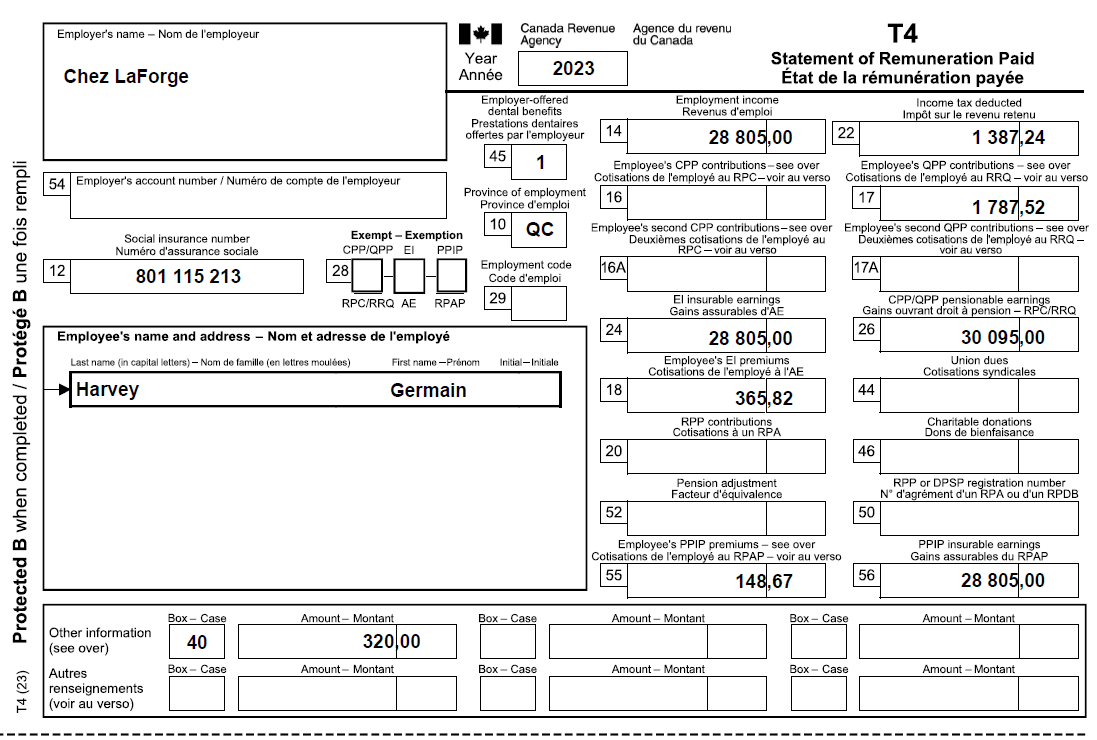
\includegraphics[width=.9\textwidth]{exercice/2-6/Q1/a-T4.png}
		\caption[]{Exercice 6, T4}
		\label{fig:Chap2Exercice6Q1T4}
	\end{figure}
	\begin{figure}
		\centering
		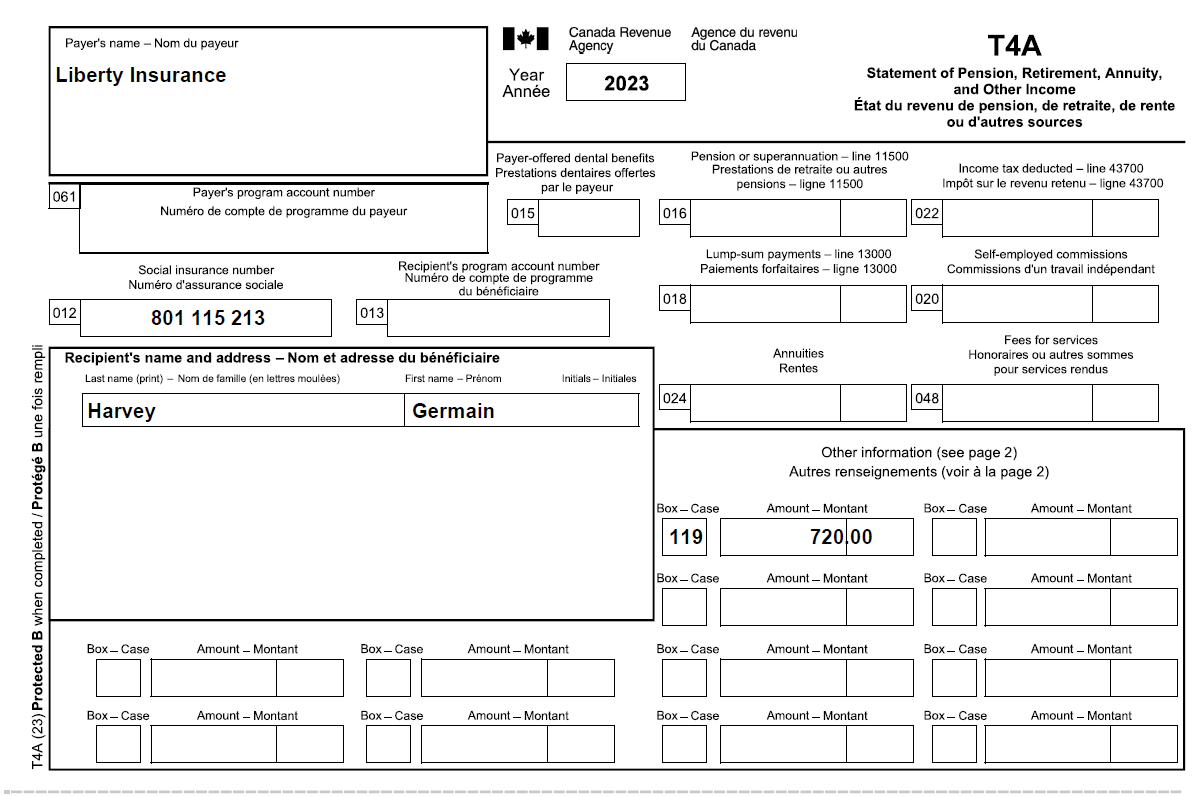
\includegraphics[width=.9\textwidth]{exercice/2-6/Q1/a-T4A.png}
		\caption[]{Exercice 6, T4A}
		\label{fig:Chap2Exercice6Q1T4A}
	\end{figure}
\end{sousQuestion}
Réponse: figure \ref{fig:Chap2Exercice6Q1aReponse}.
\begin{figure}
	\centering
	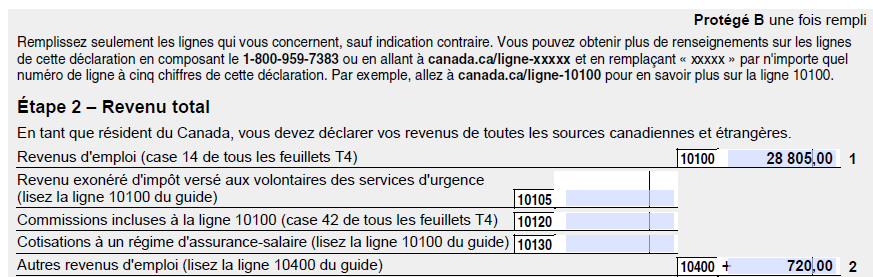
\includegraphics[width=.9\textwidth]{exercice/2-6/Q1/a-reponse.png}
	\caption[]{Exercice 6, T1}
	\label{fig:Chap2Exercice6Q1aReponse}
\end{figure}

\begin{sousQuestion}
	Germain Harvey a également reçu les feuillets Relevés~1 et 22 (figures \ref{fig:Chap2Exercice6Q1RL1} et \ref{fig:Chap2Exercice6Q1RL22}). Effectuez la correction de son revenu d'emploi à l'aide de la grille de calcul 105. Inscrivez les montants aux cases et lignes de 94 à 105 qui doivent être remplies sur la TP-1
	\begin{figure}
		\centering
		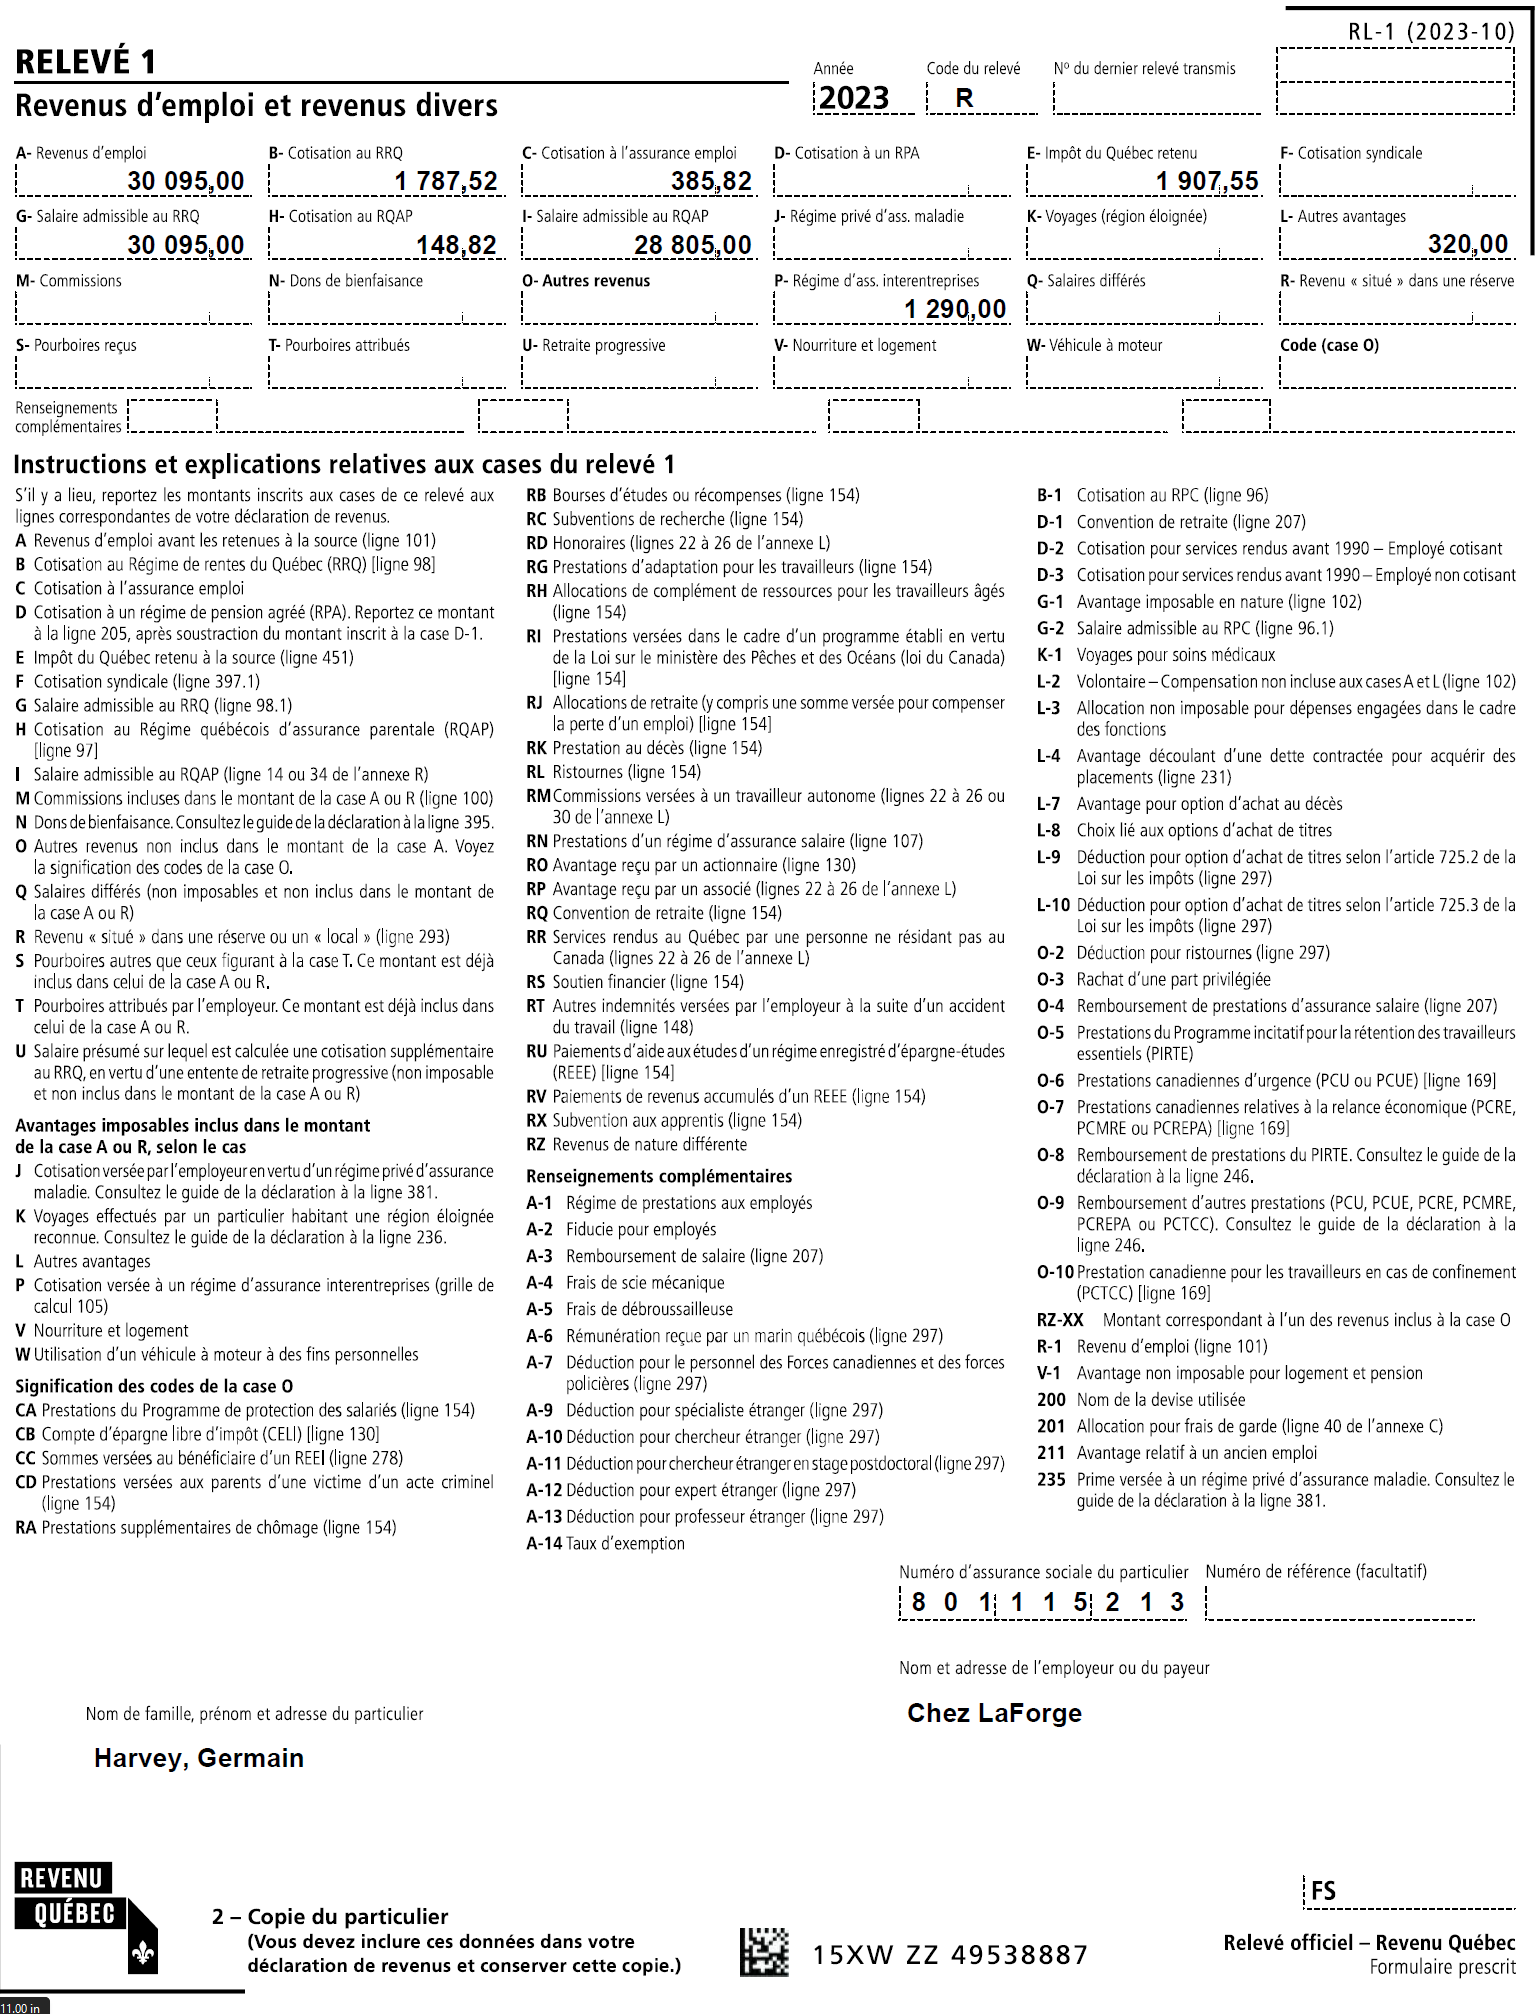
\includegraphics[width=.9\textwidth]{exercice/2-6/Q1/b-RL1.png}
		\caption[]{Exercice 6, RL-1}
		\label{fig:Chap2Exercice6Q1RL1}
	\end{figure}
	\begin{figure}
		\centering
		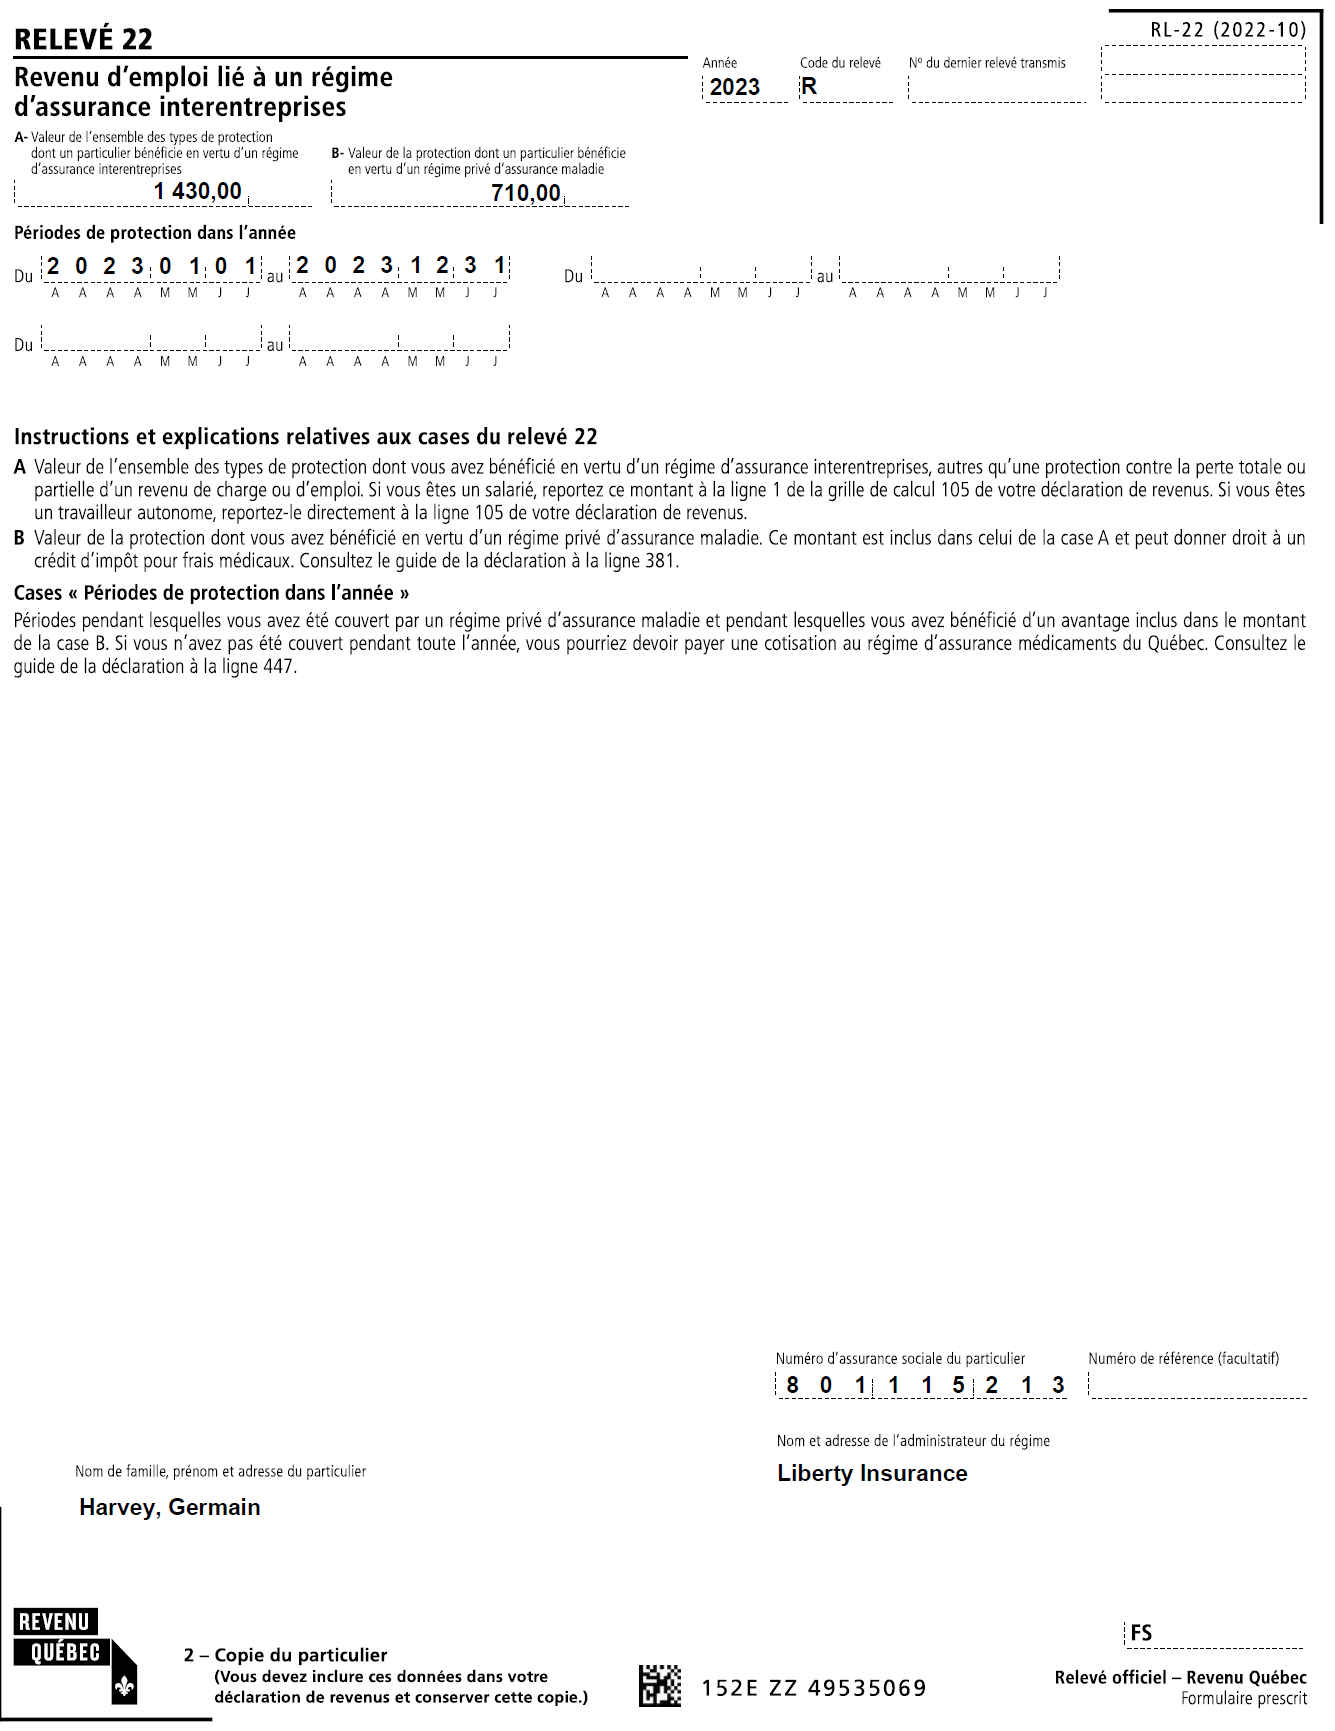
\includegraphics[width=.9\textwidth]{exercice/2-6/Q1/b-RL22.png}
		\caption[]{Exercice 6, RL-22}
		\label{fig:Chap2Exercice6Q1RL22}
	\end{figure}
\end{sousQuestion}
Réponse: figures \ref{fig:Chap2Exercice6Q1b105Reponse} et \ref{fig:Chap2Exercice6Q1bTP1Reponse}.
\begin{figure}
	\centering
	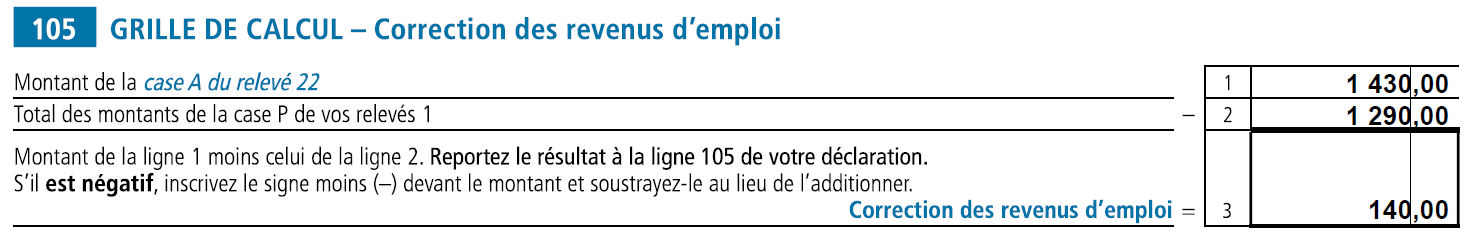
\includegraphics[width=.9\textwidth]{exercice/2-6/Q1/b-105-reponse.png}
	\caption[]{Exercice 6, Grille de calcul~105}
	\label{fig:Chap2Exercice6Q1b105Reponse}
\end{figure}
\begin{figure}
	\centering
	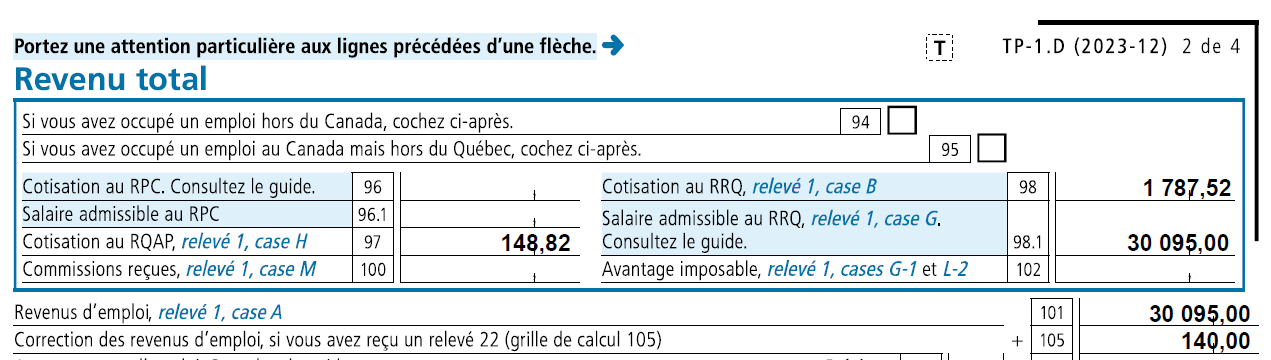
\includegraphics[width=.9\textwidth]{exercice/2-6/Q1/b-TP1-reponse.png}
	\caption[]{Exercice 6, TP-1}
	\label{fig:Chap2Exercice6Q1bTP1Reponse}
\end{figure}

\begin{question}
	Thomas Gagné a reçu deux T4(figures \ref{fig:Chap2Exercice6Q2T4numero1} et \ref{fig:Chap2Exercice6Q2T4numero2}). Quel montant doit-il inscrire aux lignes~10100 et 10120 de sa T1?
	\begin{figure}
		\centering
		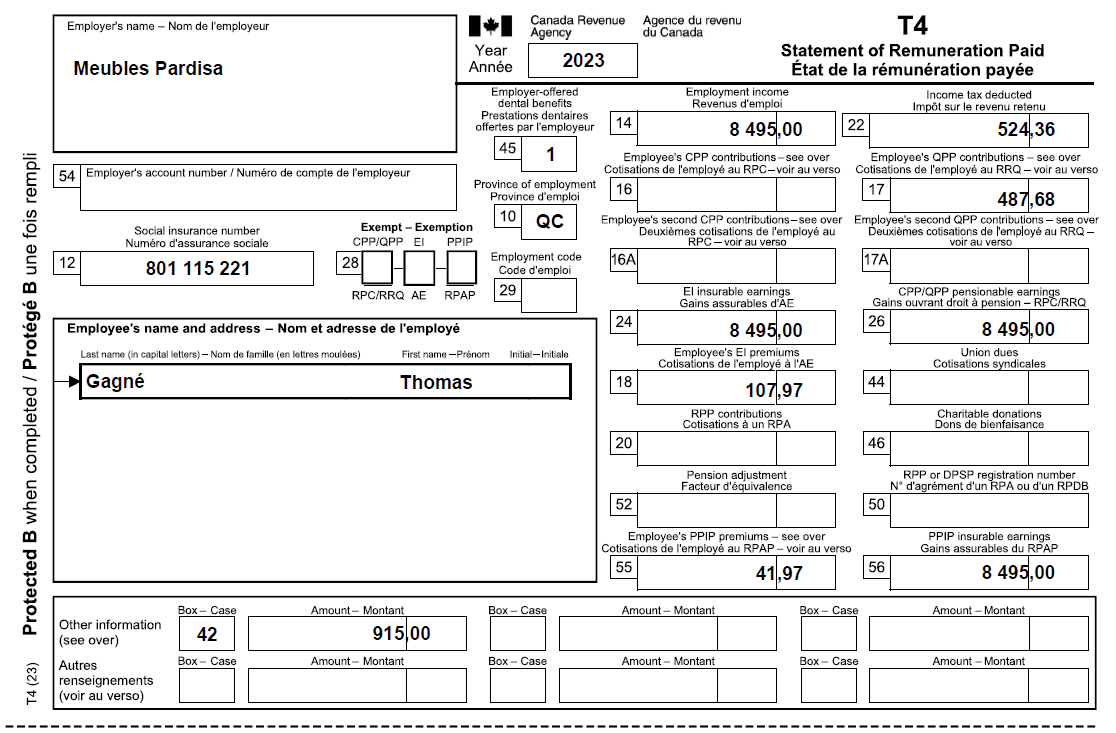
\includegraphics[width=.9\textwidth]{exercice/2-6/Q2/T4-1.png}
		\caption[]{Exercice 6, T4 Meubles Pardisa}
		\label{fig:Chap2Exercice6Q2T4numero1}
	\end{figure}
	\begin{figure}
		\centering
		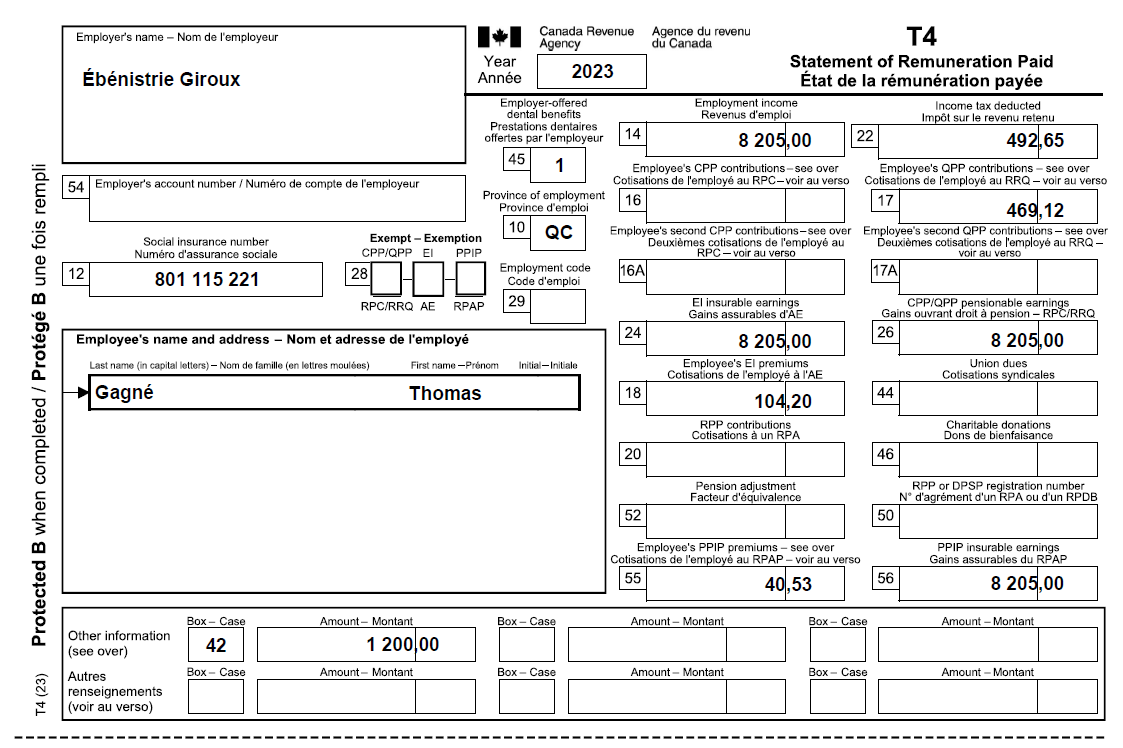
\includegraphics[width=.9\textwidth]{exercice/2-6/Q2/T4-2.png}
		\caption[]{Exercice 6, T4 Ébénisterie Giroux}
		\label{fig:Chap2Exercice6Q2T4numero2}
	\end{figure}
\end{question}
\[ \text{ligne~10100} = 8495 + 8205 = 16700\]
\[ \text{ligne~10120} = 915 + 1200 = 2115\]

\begin{question}
	Certains revenus d'emploi sont reportés aux lignes~10100 de la T1 et 101 de la TP-1, tandis que d'autres sont reportés aux lignes~10400 de la T1 et 107 de la TP-1. 
	
	Si on vous a versé un revenu d'emploi, comment pouvez-vous savoir à quelle ligne vous devez le déclarer?
\end{question}
Si le revenu d'emploi est indiqué aux cases~14 du T4 et A du relevé~1, il doit être reporté aux lignes~10100 de la T1 et 101 la TP-1.

Règle générale, tous les autres revenus liés à l'emploi, qui ne figurent pas sur des feuillets, sont reportés à la ligne~10400 de la T1 et à la ligne~107, code \og 05\fg{} à la case~106, de la TP-1.

Certaines exceptions existent.
D'autres sources de revenus peuvent s'inscrire aux lignes~13000 de la T1 et 154 de la TP-1.

Si vous n'avez pas en main les endos des feuillets d'impôts, consulter alors les guides de déclarations de revenus pour en savoir plus long.

\begin{question}
	Alain a gagné un revenu d'emploi de \numprint{10300}~\$, indiqué aux cases~14 de son T4 et A de son relevé~1. Durant l'année d'imposition, il a également reçu \numprint{2350}~\$ de pourboires qui ne sont pas indiqués nulle part sur ses feuillets.
\end{question}
\setcounter{sousQuestion}{0}
\begin{sousQuestion}
	D'après Alain, il doit déclarer seulement les revenus indiqués sur des feuillets. Puisqu'il n'a aucun feuillet indiquant le montant de ses pourboires, il est convaincu qu'il n'est pas tenu de les déclarer. 
	
	Est-ce qu'il a raison? Expliquez votre réponse.
\end{sousQuestion}
Non. Alain a tort.

La loi exige que le contribuable déclare ses revenus de toutes les sources, peu importe qu'ils soient inscrits sur des feuillets ou pas, sauf pour les montants mentionnés dans le chapitre 1 qui sont spécifiquement exonérés d'impôt et exclus du revenu.

Les pourboires qui ne figurent pas sur des feuillets doivent être déclarés aux lignes~10400 de la T1 et 107, code \og 01\fg{} à la case~106, de la TP-1.

\begin{sousQuestion}
	Auxquelles lignes de la T1 et de la TP-1, les informations ci-dessus doivent-elles être déclarées. Incluez le code correspondant sur la TP-1, s'il y a lieu.
\end{sousQuestion}

\numprint{10300}~\$: T1.10100 et TP-1.101

\numprint{2350}~\$: T1.10400 et TP-1.107 + TP-1.106 = 01

\begin{question}
	Auxquelles lignes des déclarations T1 et TP-1 doivent être reportés les revenus suivants? 
	Incluez le code correspondant sur la TP-1, s'il y a lieu.
	\begin{itemize}
		\item Pourboires reçus (pas sur T4 ni RL-1)
		\item Revenus de gardiennage (2 jours par mois)
		\item Travail temporaire (850 \$)
	\end{itemize}
\end{question}
\begin{itemize}
	\item Pourboires: T1.10400, TP-1.107, TP-1.106 = 01
	\item Gardiennage d'enfants: T1.10400, TP-1.107, TP-1.106 = 05
	\item Travail temporaire: T1.10400, TP-1.107, TP-1.106 = 05
\end{itemize}



\section{Régimes d'assurance de sécurité du revenu en cas de maladie ou de perte d'emploi}
\begin{intro}
	Il existe différents types de régimes de maladie, d'accident, d'invalidité et de maternité qui fournissent des prestations aux employés en raison de la perte de revenus lorsqu'ils sont malades, blessés, invalides, enceintes ou licenciés.
	
	Il s'agit de régimes privés, qui ne relèvent ni du Régime des rentes du Québec ni du régime fédéral d'assurance-emploi. 
	
	Les revenus ou les prestations de ces régimes peuvent être entièrement imposables, partiellement imposables ou exonérés d'impôt.
\end{intro}


\subsection{Prestation d'assurance salaire ou prestation d'assurance collective contre la maladie ou les accidents}
\begin{enumerate}
	\item L'employeur a payé toutes les cotisations
	\begin{enumerate}
		\item Si l'employeur finance le régime, exerce un contrôle et détermine les critères d'admissibilité, alors les prestations seront assujetties à des retenues à la source (cotisations RRQ, RQAP, assurance emploi et impôts).
		
		Il est déclaré à la ligne~10100 de la T1 et à la ligne~101 de la TP-1.
		\item Si l'employeur finance le régime, mais que celui-ci est contrôlé par un administrateur externe, l'administrateur émet alors un feuillet T4A (case~107) et un Relevé~1 (case~O, code~RN  dans la case Code (case~O) ). Ce revenu n'est pas assujetti aux déductions pour le RRQ, l'AE ou le RQAP.
		
		Le montant total reçu est imposable et doit être déclaré aux lignes~10400 de la T1 et 107, code~02 à la case~106 de la TP-1.
	\end{enumerate}
	\item L'employé a payé toutes les cotisations, aucun feuillet ne sera émis, car aucun des avantages reçus n'est imposable. Le montant reçu n'a pas à être inscrit sur les déclarations de l'employé.
	\item Si l'employeur et l'employé ont tous deux versé des primes au régime, les feuillets de renseignements émis sont similaires à ceux décrits dans l'option 1, en fonction de la personne qui exerce le contrôle sur le plan.
	\begin{enumerate}
		\item Si l'employeur exerce un contrôle sur le régime, le revenu est inclus dans la case~14 du T4 et dans la case~A du Relevé-1
		
		Toutefois, l'employé peut soustraire de la ligne~10100 de la T1 et de la ligne~101 de la TP-1 tout ou partie des primes inutilisées qu'il a versées au régime. Parallèlement, ce montant de réduction doit être inscrit à la ligne~10130 de la déclaration T1.
		\item Si le régime est contrôlé par un administrateur externe, celui-ci émet un feuillet T4A et un Relevé~1 (case~O, code~RN  dans la case Code (case~O)).
		
		Dans ce cas, l'employé peut soustraire la totalité ou une partie de ses primes inutilisées du montant inscrit à la case~107 du T4A et inscrire le montant réduit à la ligne~10400 de la T1. De même, le montant de la case~O du Relevé~1 est réduit en conséquence et reporté à la ligne~107, code \og 02\fg{} de la case~106 du TP-1. Notez que dans cette situation, il n'y a pas de ligne équivalente à la ligne~10130 cependant, la ligne~165 est utilisée sur le TP-1 pour inscrire les primes utilisées en tant que réduction.
	\end{enumerate}
\end{enumerate}

\subsubsection{Régime de prestations supplémentaires de chômage}
Les avantages imposables de ce régime enregistré figurent sur un T4A à la case~152. Au Québec, ils sont inscrits à la case~O du Relevé1 et le code~RA se trouve à la case Code (case~O) du Relevé1. Le montant doit être déclaré aux lignes~10400 de la T1 et 154, le code~03  à la case~153 de la TP-1.

Si un régime de prestations supplémentaires de chômage n'est pas inscrit au Programme de prestations supplémentaires de chômage (PSC), les montants versés sont inclus dans les cases~14 du T4 et A du Relevé~1. Ils doivent ensuite être déclarés à la ligne~10100 de la T1 et à la ligne~101 de la TP-1 des déclarations de revenus en tant que revenus d'emploi.

\subsubsection{Régime de participation des employés aux bénéfices}
Dans la déclaration fédérale, ces montants reçus sont indiqués à la case~35 Autres revenus d'emploi du feuillet T4PS. Ils doivent être déclarés à la ligne~10400 de la déclaration T1.

Au Québec, on regarde si le revenu est assujetti ou non à une cotisation au RRQ. Ceci est déterminé par les cases Renseignements complémentaires du Relevé~25 comme suit:

Inscrivez à la ligne~101 de la déclaration TP-1, si le montant figure également à la case~D-1 du Relevé~25. Ce montant fait l'objet d'une cotisation au RRQ.
Inscrivez à la ligne~107, code~03 à la case~106 de la TP-1 si le montant figure également à la case~D-2 du Relevé~25. Ce montant n'est pas assujetti à une cotisation au RRQ.

\begin{note}
	Ces régimes peuvent inclure des dividendes, des gains en capital, et des revenus de source étrangère.
\end{note}

\subsubsection{Paiements provenant du programme de protection des salariés}
Dans la déclaration fédérale, le montant figure à la case~132 du T4A. Au Québec, il figure à la case~O du Relevé1, avec le code~CA dans la case  Code (case~O). Il doit être déclaré aux lignes~10400 de la T1 et 154, code~12 à la case~153 de la TP-1.



\section{Subventions et redevances}
\begin{intro}
	Les subventions permettant de mener des recherches, les subventions en reconnaissance d'une réalisation et certaines redevances sont considérées comme d'autres revenus d'emploi.
\end{intro}


\subsection{Subventions de recherche}
Lorsque l'employeur verse la subvention, toute portion qui représente un revenu est déclarée sur un T4 et un Relevé~1.

Sinon, la subvention est déclarée à la case~104 du T4A et à la case~O du Relevé~1. Comme la case~O est utilisée pour de nombreux types de revenus, une information supplémentaire est fournie dans la case Code (case~O) pour indiquer le type de revenu reçu. Pour les subventions de recherche, le code est RC. 

Le contribuable qui a reçu une subvention de recherche peut déduire les dépenses payées ou encourues pour la réalisation de son projet:
\begin{itemize}
	\item Frais de déplacement (y compris les repas et l'hébergement) pour les voyages de recherche
	\item Frais de laboratoire
	\item Achat d'équipement/de fournitures
	\item Salaire versé à un assistant
\end{itemize}

Les dépenses suivantes ne sont pas déductibles:
\begin{itemize}
	\item Les dépenses personnelles et de subsistance, autres que les frais de déménagement
	\item Les dépenses pour lesquelles le contribuable a reçu un remboursement, à moins que le remboursement ne soit inclus dans la subvention
	\item Les coûts déductibles déjà pris en compte dans le calcul du revenu
\end{itemize}

\rqg{30 \S j}


\subsection{Subvention incitative aux apprentis (SIA)}
Déclaré à la case~130 du T4A. Inscrit à la ligne~13000 de la T1. Déclaré dans la case~O du Relevé~1 en utilisant le code~RX. Inscrit à la ligne~154 de la TP-1 en utilisant le code~03.


\subsection{Subvention à l'achèvement de la formation d'apprenti (SAFA)}
Déclaré à la case~130 du T4A. Inscrit à la ligne~13000 de la T1. Déclaré dans la case~O du Relevé~1 en utilisant le code~RX. Inscrit à la ligne~154 de la TP-1 en utilisant le code~03.

\cat\href{https://www.red-seal.ca/fra/w.2lc.4m.2.shtml}{Programme Sceau rouge}


\subsection{Redevances provenant d'une œuvre ou d'une invention}
Ces redevances sont inscrites à la case~17 du T5, État des revenus de placements, et à la case~H du Relevé~3, Revenus de placements.

Au niveau fédéral, il existe différents traitements: 
\begin{itemize}
	\item Si elles sont reçues pour un travail ou une invention du contribuable, les redevances doivent être déclarées à la ligne~10400 de la T1, c'est-à-dire en tant qu'autres revenus d'emploi.
	\item Sinon, elles doivent être déclarées à la ligne~12100, qui est classée comme Intérêts et autres revenus d'investissement.
\end{itemize}

Au Québec, les deux doivent être déclarés à la ligne~130 de la TP-1 en tant qu'intérêts et autres revenus d'investissement.



\section{Revenu total}
En supposant que le contribuable n'a aucun autre revenu, on inscrit le total des lignes~10100, 10400 et 13000 à la ligne~15000 de la T1.

Au Québec, c'est à la ligne~199 qu'on doit inscrire le total des lignes~101, 105, 107 et 154.



\section{Exercice 7}
\setcounter{question}{0}
\begin{question}
	Roger a été en arrêt de travail pour cause de maladie pendant une période de quatre mois.
	
	Son T4A et son Relevé~1 indiquent qu'il a reçu \numprint{1600}~\$ en prestations d'un régime d'assurance-salaire. Il a versé des cotisations annuelles de \numprint{200}~\$ au régime au cours des cinq dernières années. Son employeur a également cotisé au régime au cours de chacune de ces années, mais il n'exerce pas de contrôle. 
	
	Dans l'espace ci-dessous, calculez le montant et indiquez sur quelles lignes ce montant doit être inscrit sur les déclarations T1 et TP1 de Roger, en supposant qu'il s'agit de la première année où il a reçu des prestations du régime.
\end{question}
Le calcul doit être effectué comme suit:

\begin{itemize}
	\item Montant reçu (T4A et Relevé~1): \numprint{1600}~\$
	\item Moins: total des cotisations de l'employé versées au régime (5 x 200~\$): \numprint{1000}~\$ 
	\item Montant à déclarer à la ligne~10400 de la T1 et à la ligne~107 de la TP-1, en utilisant le code~02 à la case~106: 600~\$
\end{itemize}

Les primes soustraites de la prestation doivent être inscrites à la ligne~165 du formulaire TP-1.

\begin{question}
	Gilles Fortin est professeur à l'Université de Montréal. Au cours de l'année d'imposition, il a reçu une subvention de recherche de \numprint{38000}~\$ de l'université, pour laquelle il a reçu un T4A et un
	Relevé~1.
	
	Il a payé un assistant \numprint{10000}~\$ pour effectuer une partie de la recherche.
	Si le Dr Fortin n'a pas d'autres dépenses applicables, quel montant de la subvention de recherche doit-il déclarer dans sa déclaration, et sur quelles lignes?
\end{question}
Il doit déclarer le montant net de la subvention, c'est-à-dire la subvention moins les dépenses admissibles. Il doit donc inscrire \numprint{28000}~\$ (\numprint{38000}~\$ $-$ \numprint{10000}~\$) à la ligne~10400 de la T1 et à la ligne~154 de la TP-1, avec le code~03 à la case~153.



\section{Sommaire du chapitre}
\begin{itemize}
	\item La section d'identification de la Déclaration de revenus et de prestations et de la Déclaration de revenus servent à identifier le contribuable et à fournir des informations personnelles qui ont une incidence sur le calcul de l'impôt.
	\item Les questions d'Élections Canada permettent à l'ARC de fournir des informations personnelles sélectionnées pour mettre à jour le Registre national des électeurs.
	\item La question relative aux biens étrangers vise à encourager le respect de l'obligation de déclarer les revenus provenant de biens étrangers déterminés.
	\item L'usage de certaines cases des principaux feuillets d'impôts, soit le T4 et le Relevé~1.
	\item Les autres revenus tels que redevances, subventions de recherche, prestations supplémentaires de chômage, etc.
	\item La demande du Crédit d'impôt pour solidarité au Québec.
	\item La différence entre un revenu d'emploi d'un salarié et celui d'un travailleur autonome.
	\item Un aperçu des différents feuillets d'impôt tels le T4A, Relevé~22.
	\item La présence de grilles de calcul pour effectuer des opérations mathématiques dont le résultat s'inscrit directement sur la déclaration, notamment la grille 105 sur la correction d'emploi.
	\item Les revenus sans feuillets de renseignements. 
	\item Les prestations d'assurance-emploi, dont les situations sont diverses.
\end{itemize}



\section{Problème de révision}
\subsection{Renseignements sur le contribuable}
Voir la table \ref{table:pb2}.
\begin{table}
	\centering
	\begin{tabular}{|c|c|c|}
		\hline
		\rowcolor{LightGreen}Description &    Contribuable \no 1    & Contribuable \no 2 \\ \hline
		              Nom                &     Daniel Chartrand     &    Lise Valois     \\ \hline
		              NAS                &       801 115 239        &    801 115 247     \\ \hline
		       Date de naissance         &       23 juin 1993       &    5 mars 1994     \\ \hline
		           État civil            &          \multicolumn{2}{c|}{Mariés}          \\ \hline
		              Sexe               &            M             &         F          \\ \hline
		     Province de résidence       &            QC            &         QC         \\ \hline
		             Langue              &            A             &         A          \\ \hline
		           Téléphone             &       418 235-6479       &    418 235-9746    \\ \hline
		        Adresse courriel         & d.chartrand@videotron.ca &       Aucune       \\ \hline
		   Consentement à l'envoi de     &           Oui            &        Non         \\
		    communications par voie      &                          &                    \\
		    électronique uniquement      &                          &                    \\ \hline
		         Correspondance          &         En ligne         &       Poste        \\ \hline
		             Régime              &        RAMQ/Privé        &     RAMQ/Privé     \\
		    d'assurance médicaments      &                          &                    \\ \hline
		            Adresse              &  \multicolumn{2}{c|}{2839, boul. Laurentien}  \\
		                                 &  \multicolumn{2}{c|}{Saguenay, QC, G8C 1V3}   \\ \hline
		     Citoyenneté canadienne      &           Oui            &        Oui         \\ \hline
		        Élections Canada         &           Oui            &        Oui         \\ \hline
		        Biens étrangers          &           Non            &        Non         \\ \hline
		             Revenu              &           Oui            &        Non         \\ \hline
	\end{tabular}
	\caption[]{Problème, renseignements sur le contribuable}
	\label{table:pb2}
\end{table}

Au cours de l'année, Daniel a reçu des prestations d'un régime d'assurance-salaire. Le couple a été couvert par la RAMQ jusqu'en juillet. À partir du mois d'août, ils ont été couverts par l'assurance collective de l'employeur de Daniel.

Feuillets d'impôts de Daniel : figures \ref{fig:pb2T4Alcan} à \ref{fig:Chap2RL1Manulife}.

\begin{figure}
	\centering
	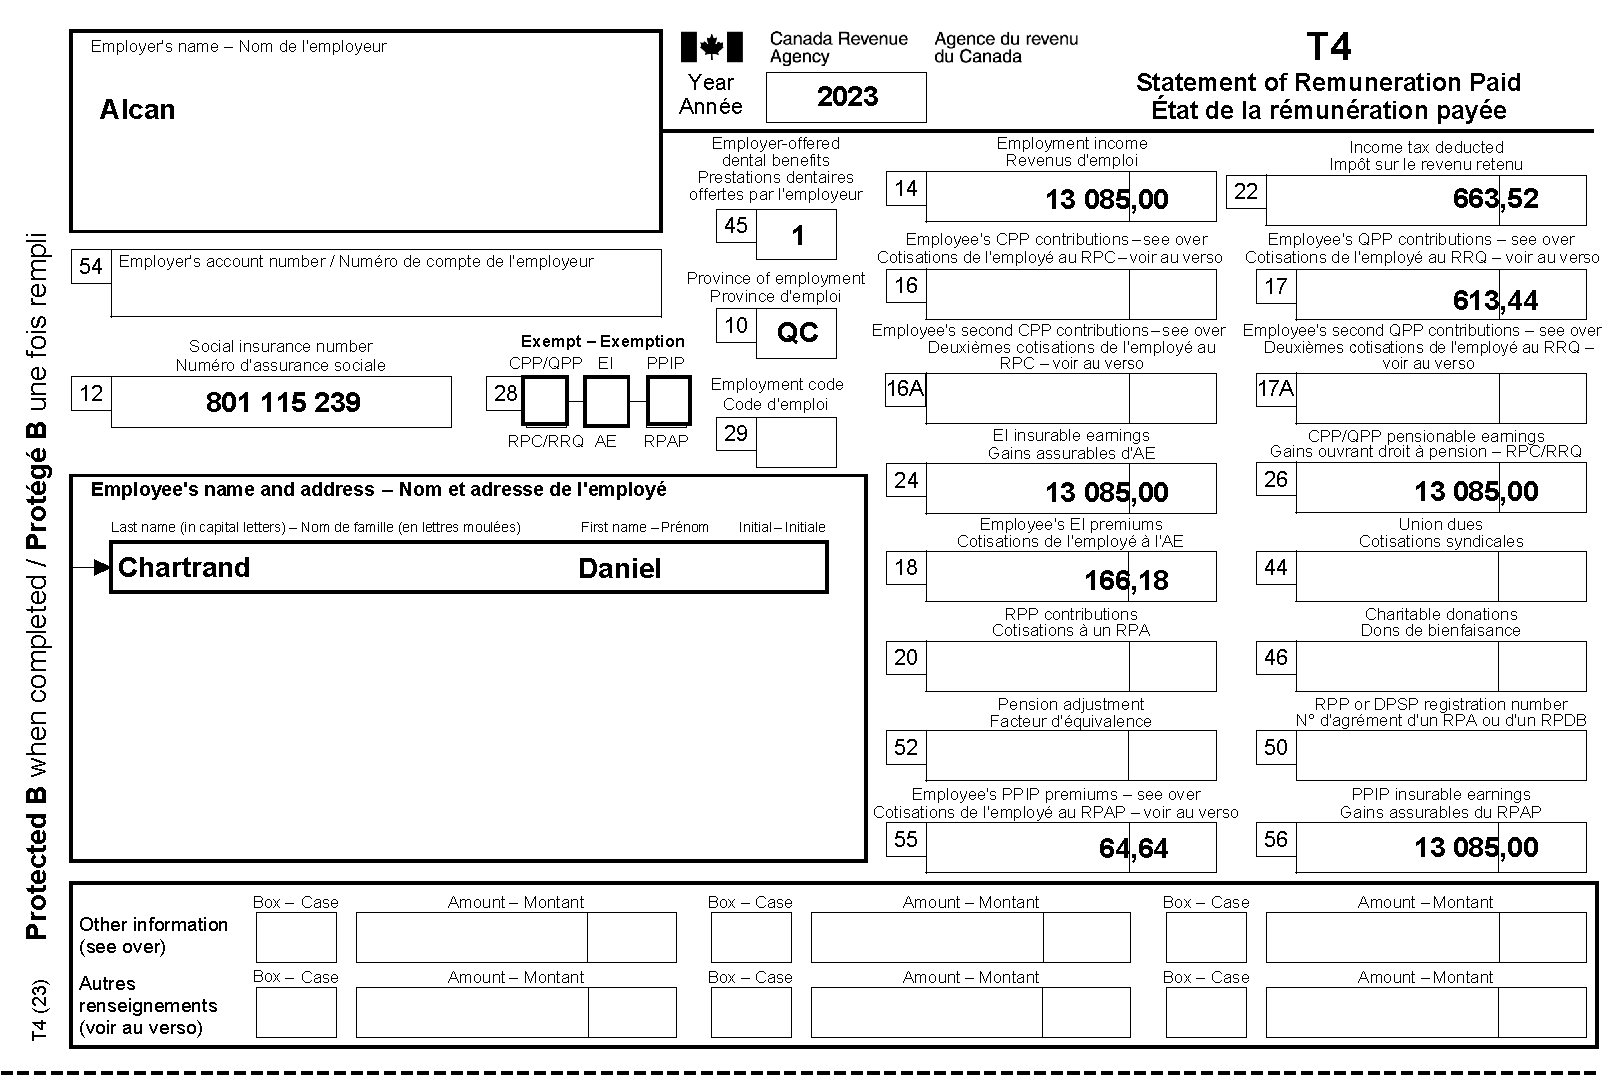
\includegraphics[width=.9\textwidth]{probleme/chapitre-2/T4-Alcan.png}
	\caption[]{Problème, T4 Alcan}
	\label{fig:pb2T4Alcan}
\end{figure}

\begin{figure}
	\centering
	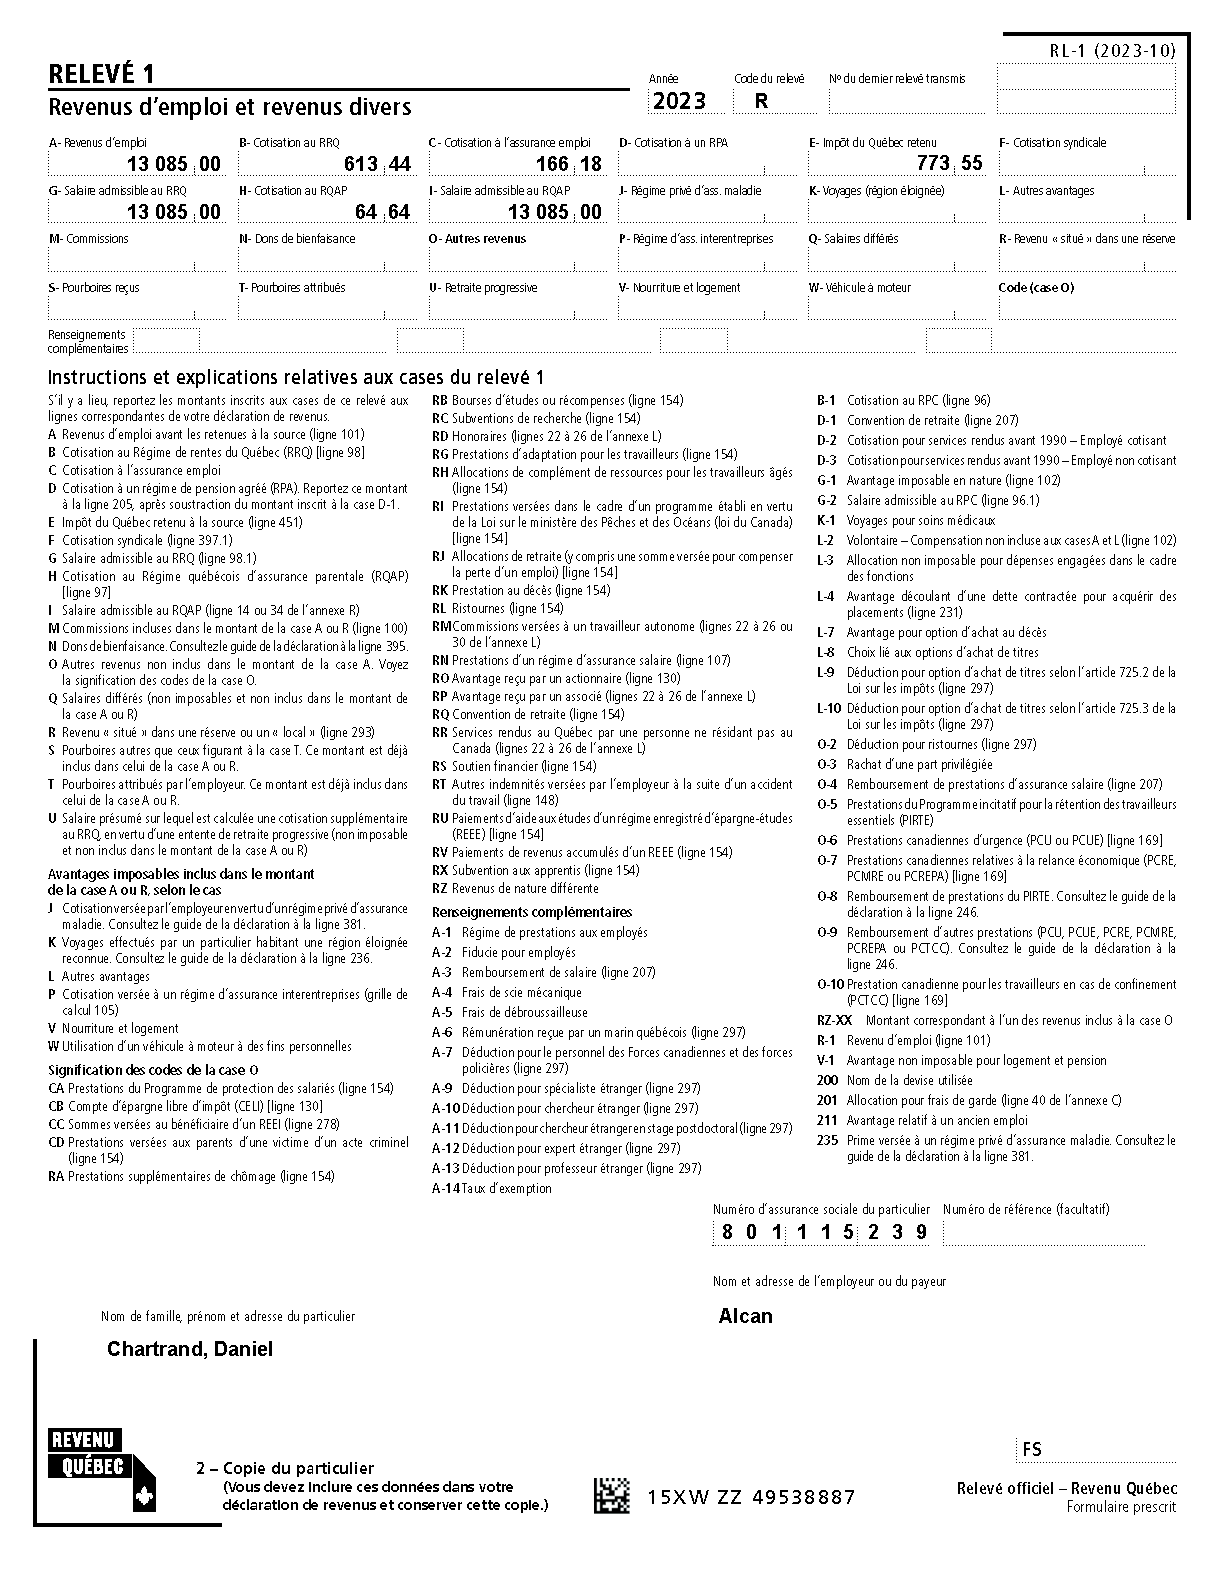
\includegraphics[width=.9\textwidth]{probleme/chapitre-2/RL1-Alcan.png}
	\caption[]{Problème, RL-1 Alcan}
	\label{fig:pb2RL1Alcan}
\end{figure}

\begin{figure}
	\centering
	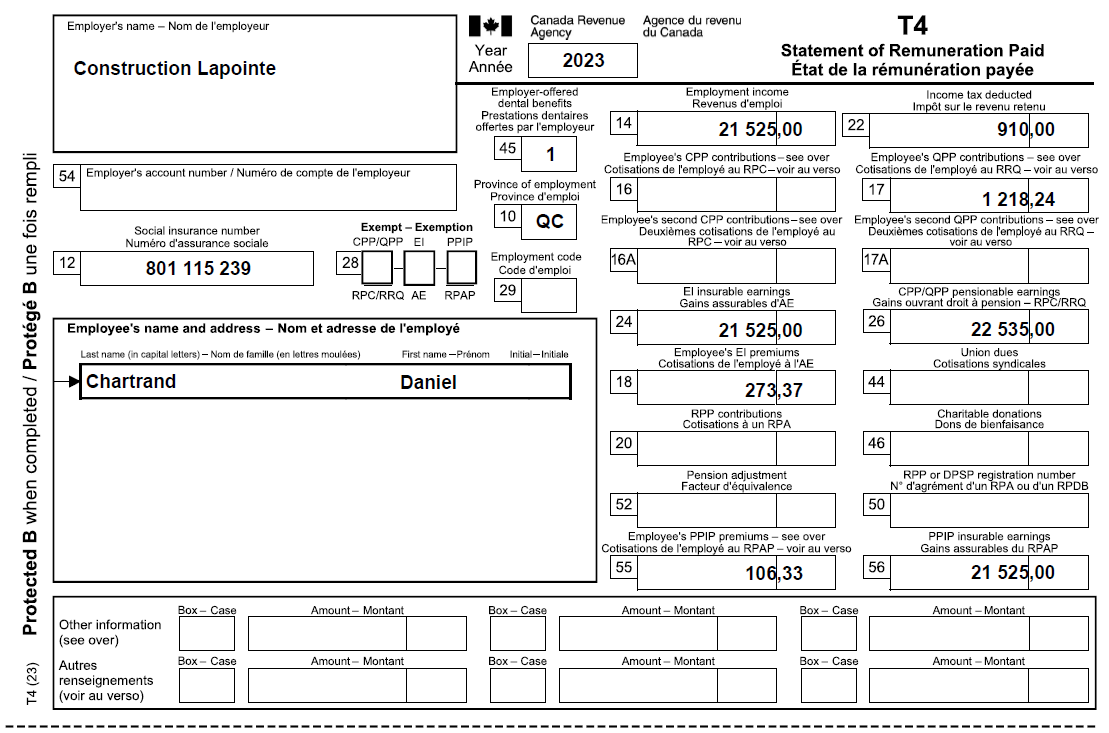
\includegraphics[width=.9\textwidth]{probleme/chapitre-2/T4-ConstructionLapointe.png}
	\caption[]{Problème, T4 Construction Lapointe}
	\label{fig:pb2T4ConstructionLapointe}
\end{figure}

\begin{figure}
	\centering
	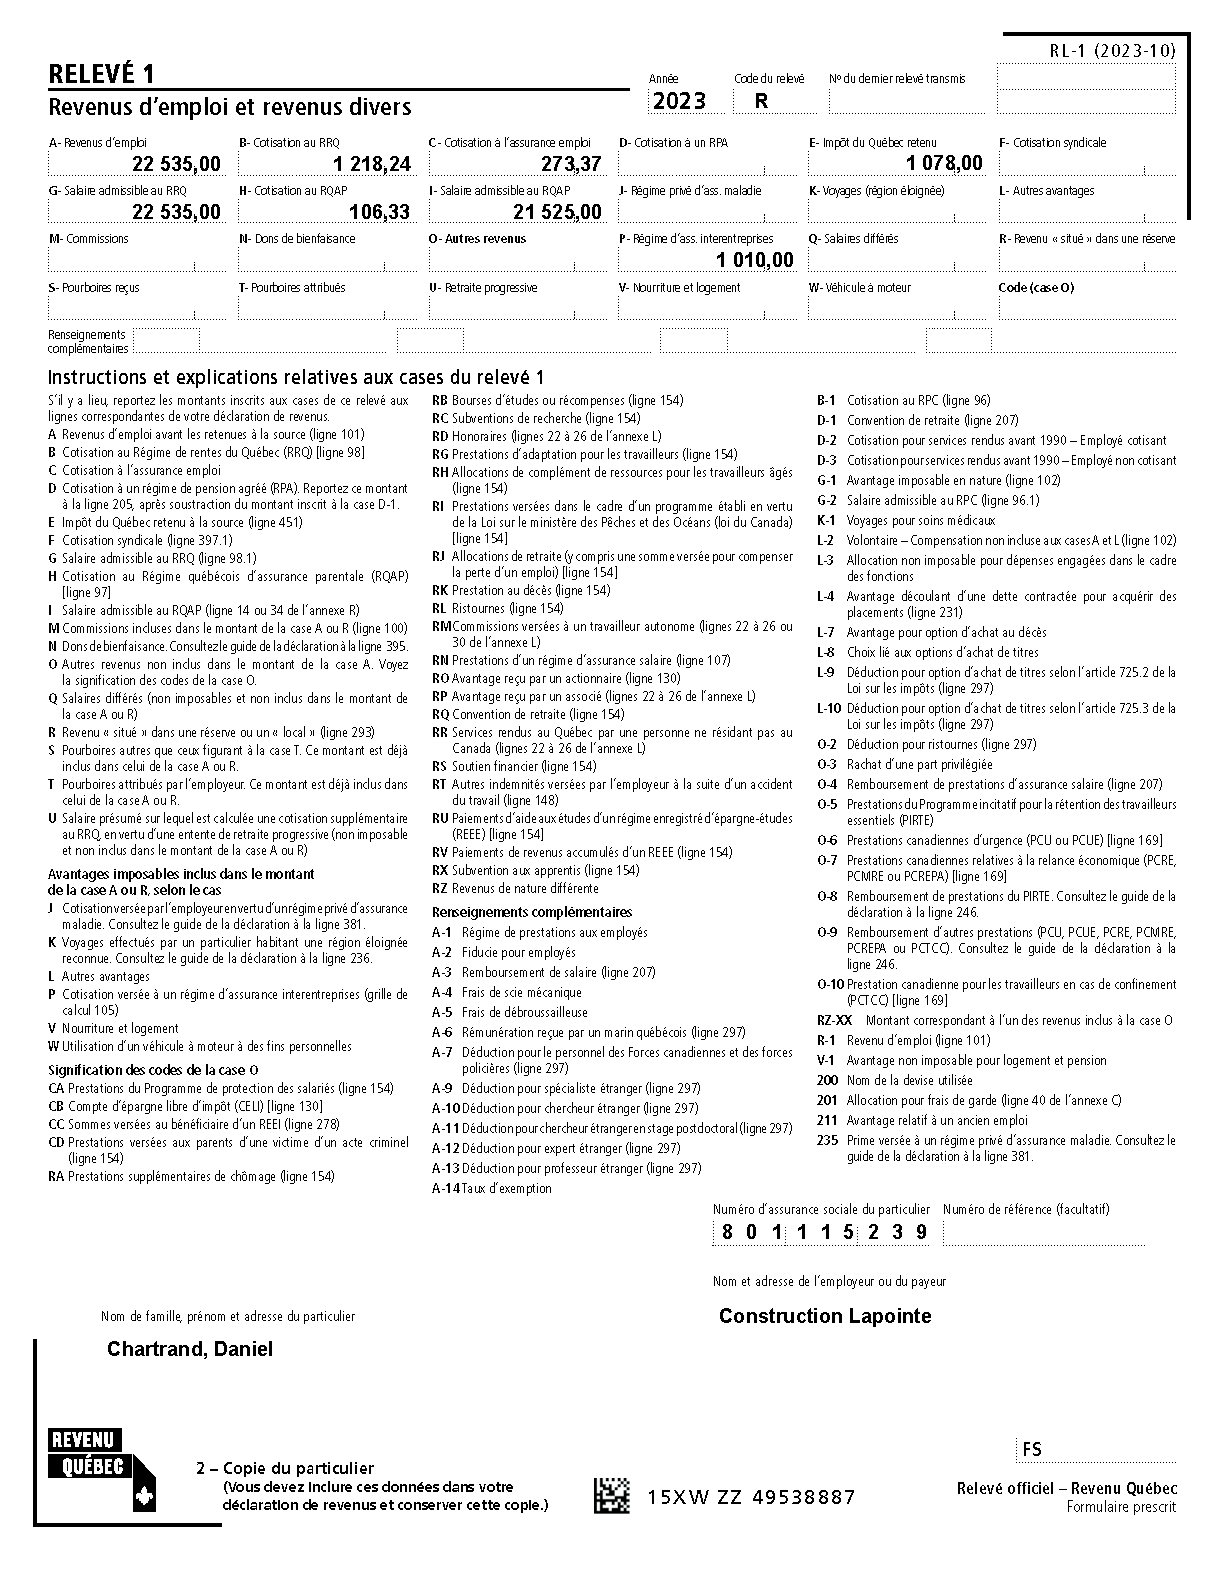
\includegraphics[width=.9\textwidth]{probleme/chapitre-2/RL1-ConstructionLapointe.png}
	\caption[]{Problème, RL-1 Construction Lapointe}
	\label{fig:pb2RL1ConstructionLapointe}
\end{figure}

\begin{figure}
	\centering
	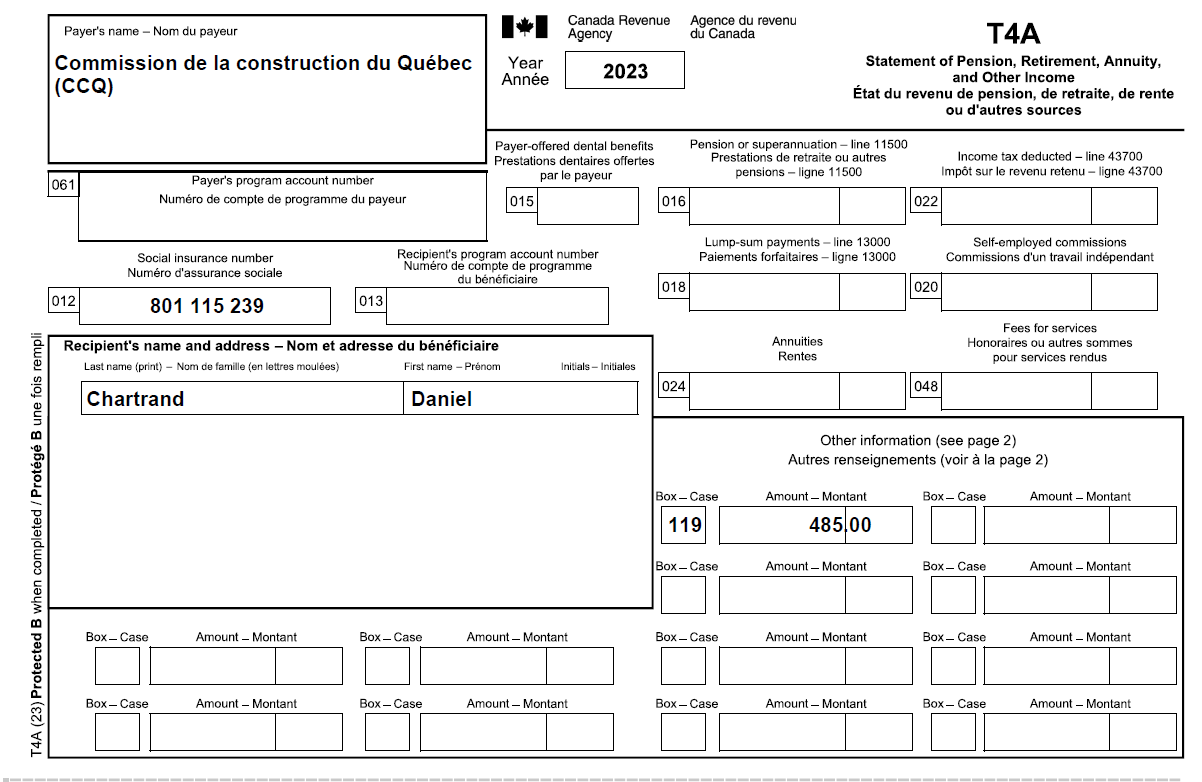
\includegraphics[width=.9\textwidth]{probleme/chapitre-2/T4A-CCQ.png}
	\caption[]{Problème, T4A CCQ}
	\label{fig:Chap2T4ACCQ}
\end{figure}

\begin{figure}
	\centering
	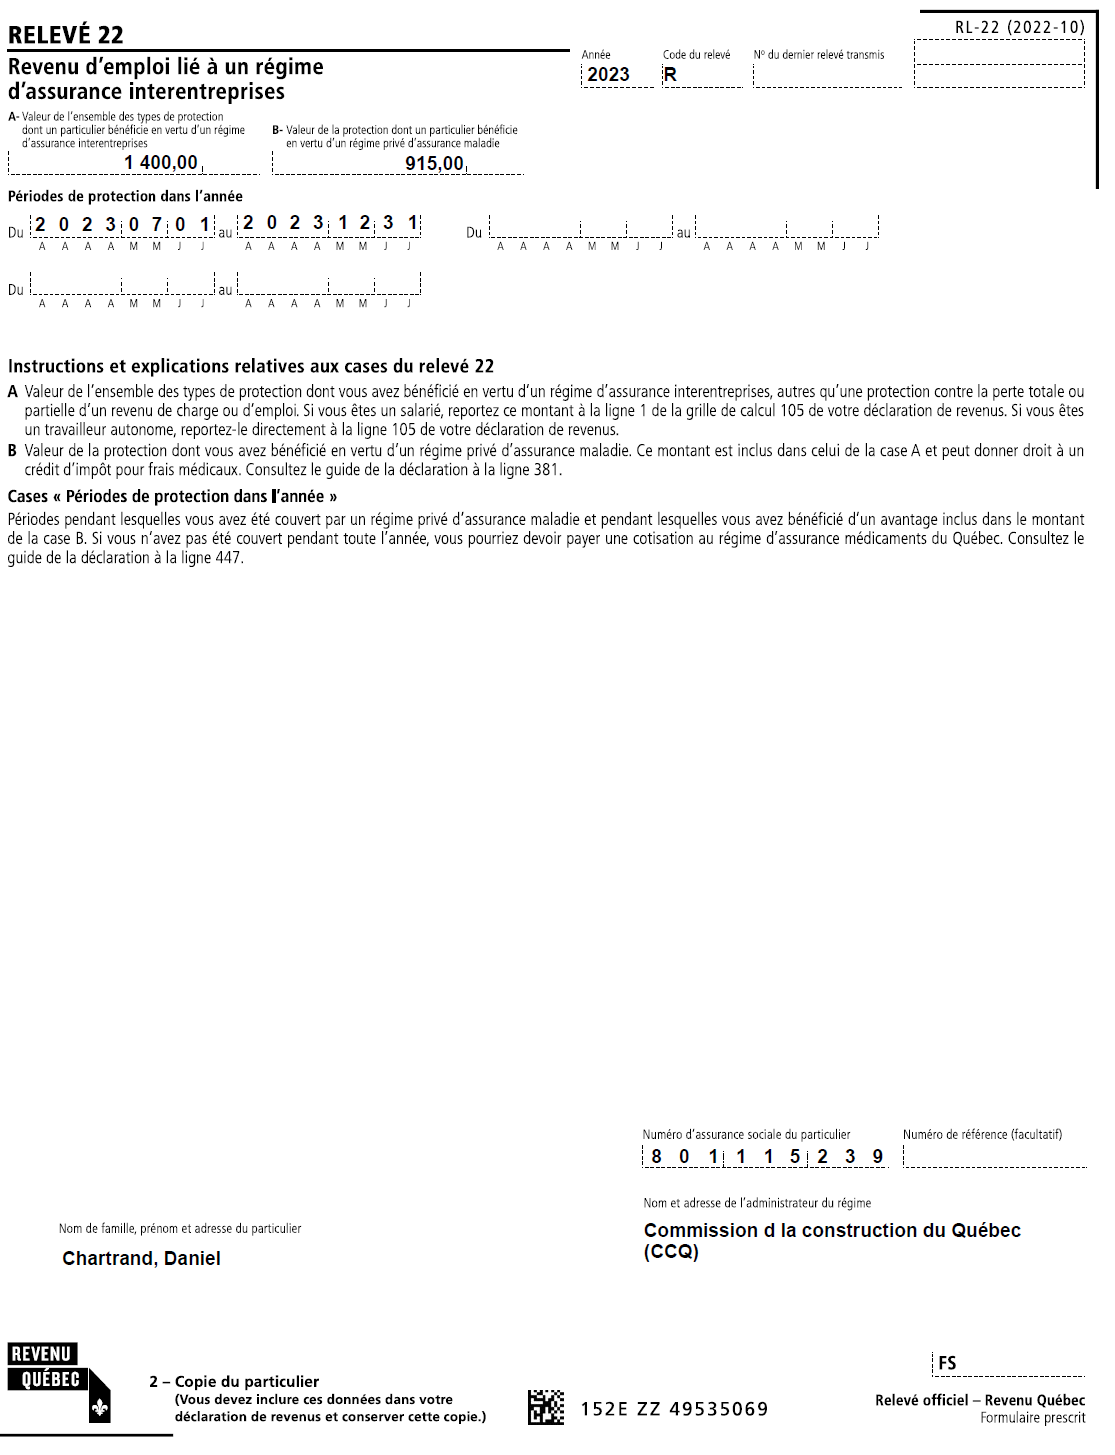
\includegraphics[width=.9\textwidth]{probleme/chapitre-2/RL22-CCQ.png}
	\caption[]{Problème, RL-22 CCQ}
	\label{fig:Chap2RL22CCQ}
\end{figure}

\begin{figure}
	\centering
	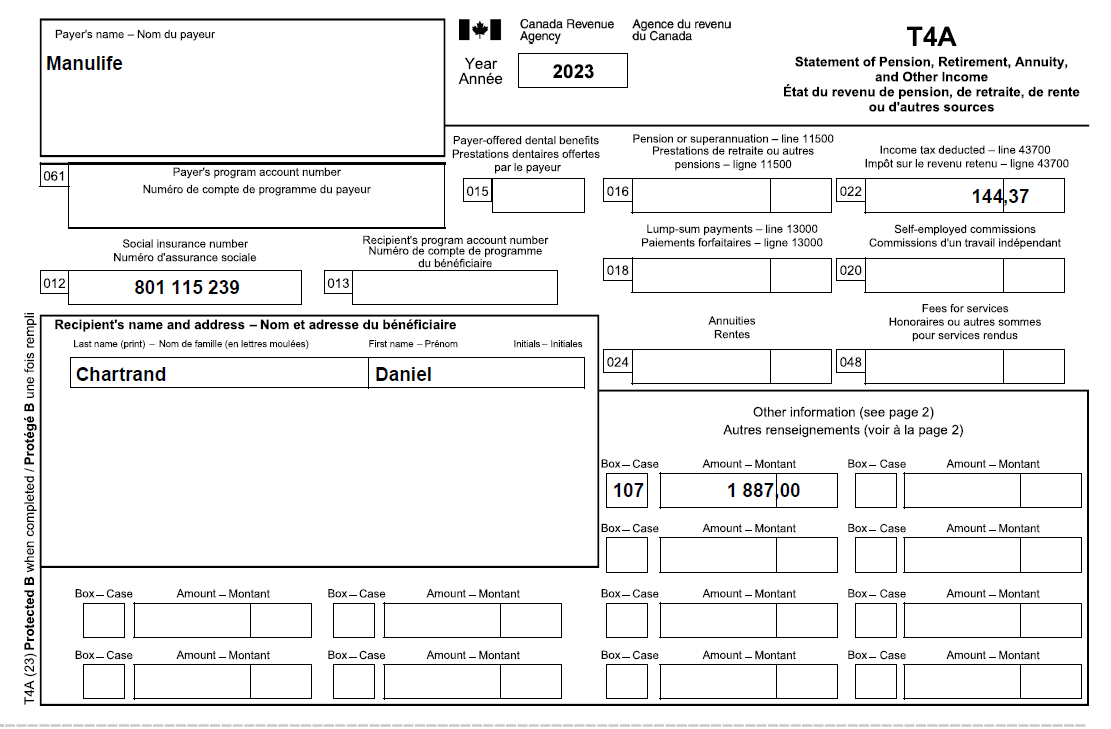
\includegraphics[width=.9\textwidth]{probleme/chapitre-2/T4A-Manulife.png}
	\caption[]{Problème, T4A Manulife}
	\label{fig:Chap2T4AManulife}
\end{figure}

\begin{figure}
	\centering
	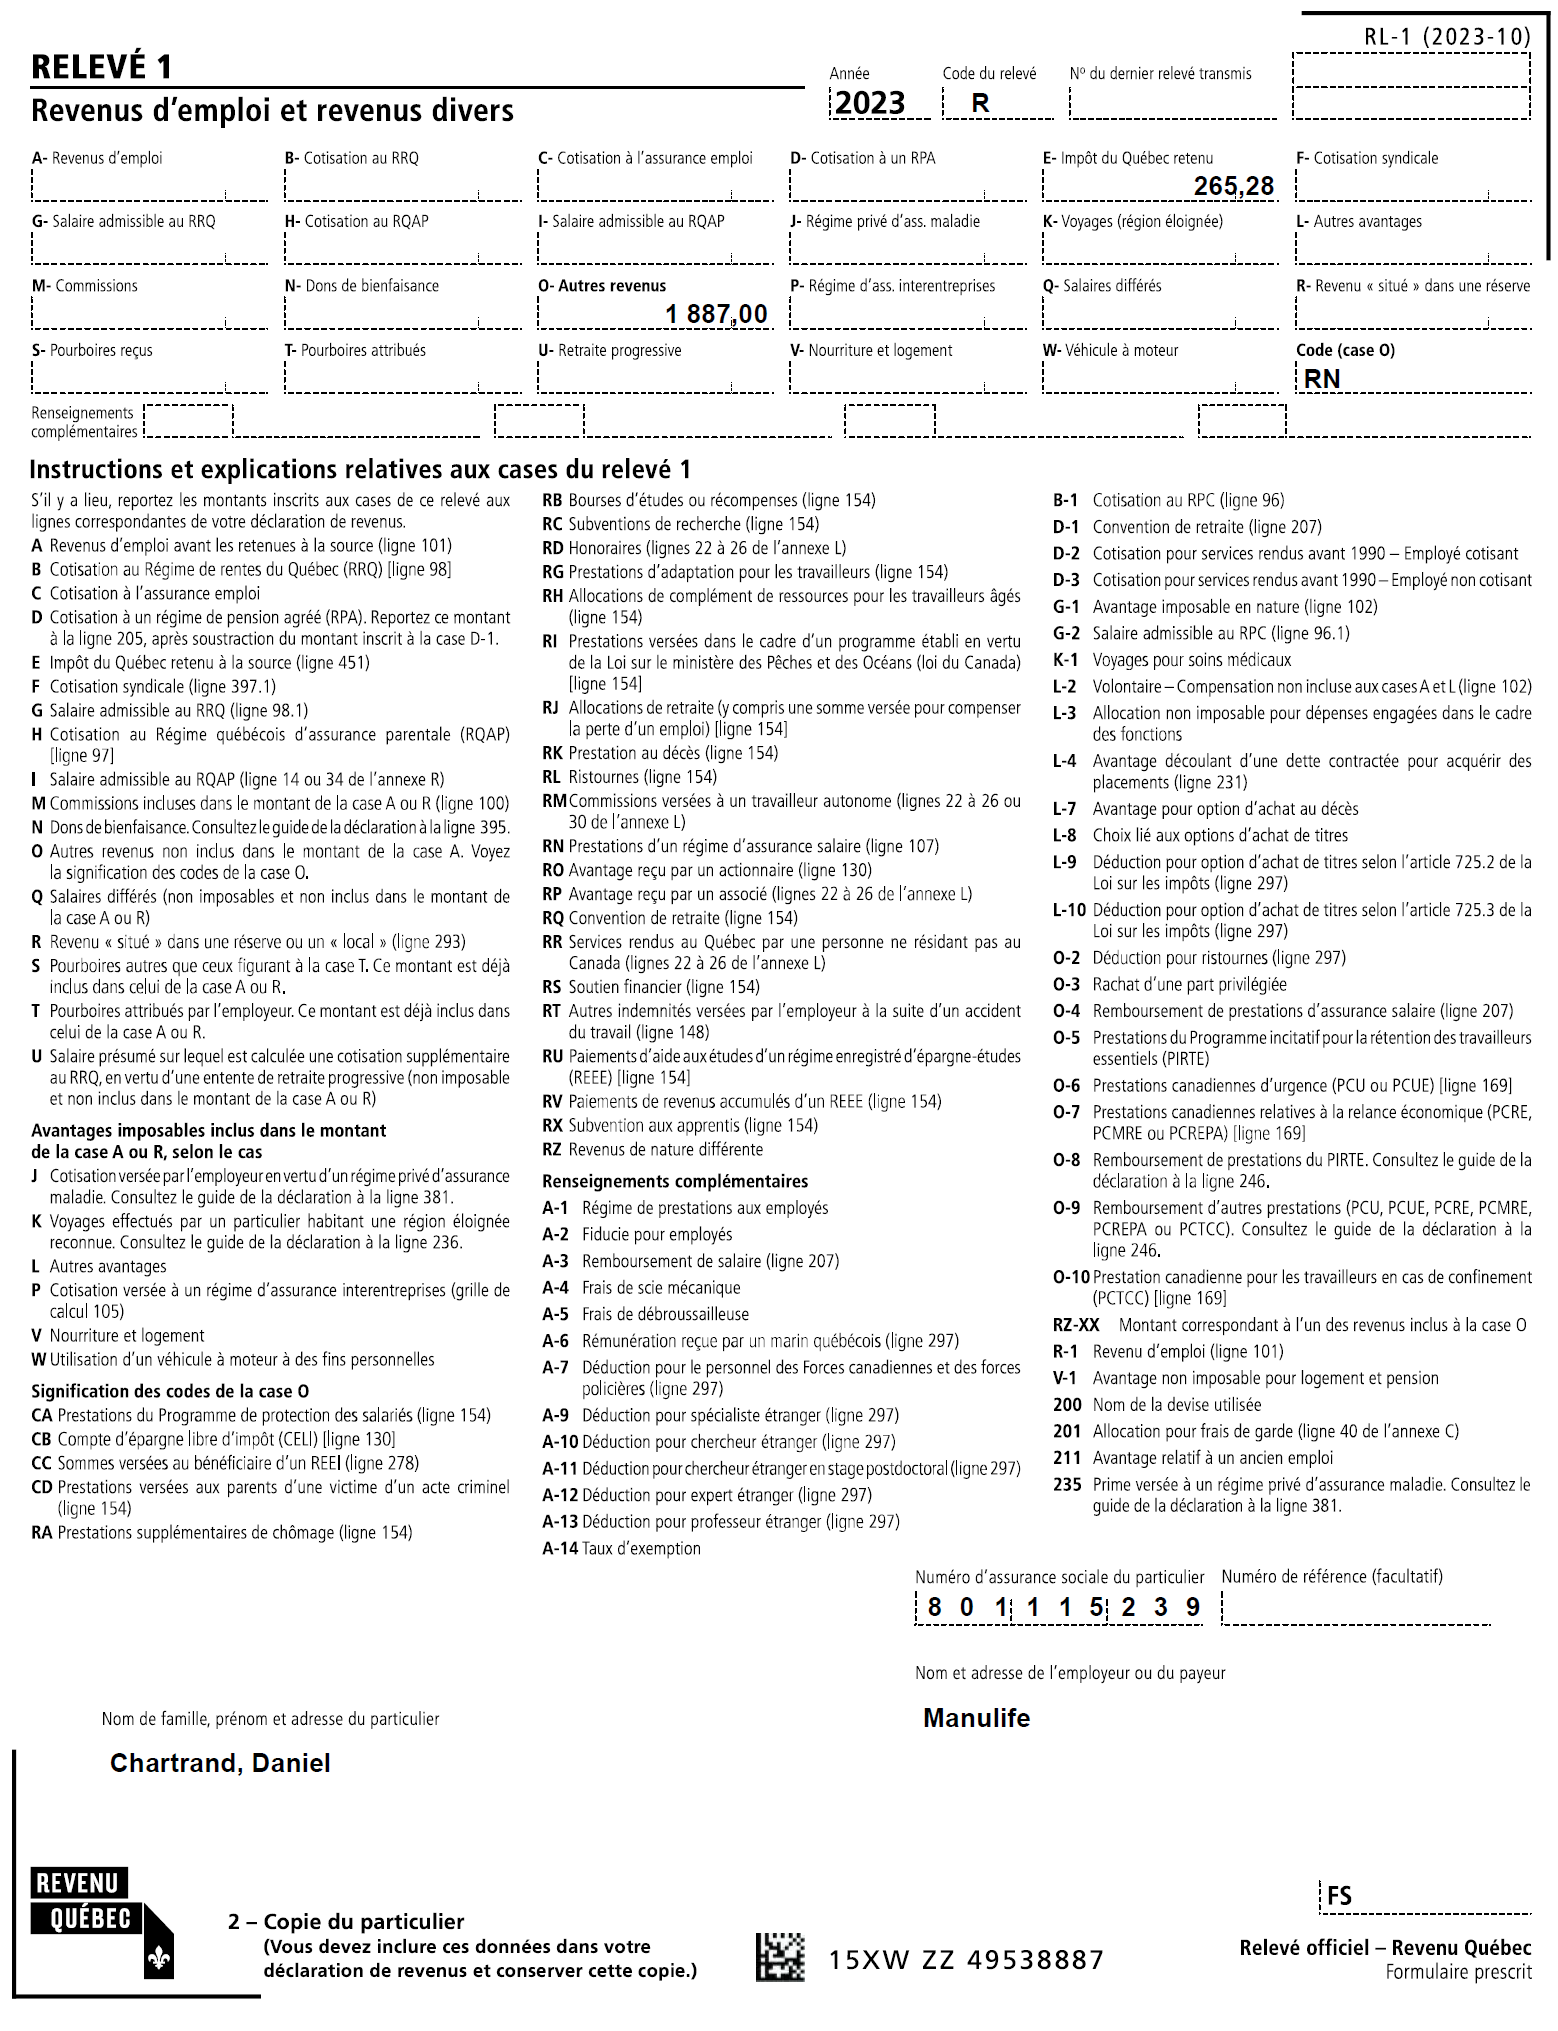
\includegraphics[width=.9\textwidth]{probleme/chapitre-2/RL1-Manulife.png}
	\caption[]{Problème, RL-1 Manulife}
	\label{fig:Chap2RL1Manulife}
\end{figure}


\setcounter{question}{0}
\begin{question}
	En quoi consiste le montant indiqué à la case~107 du T4A?
\end{question}
Paiements reçus d'un régime d'assurance-salaire payé par l'employeur.

\numprint{1887,00}~\$ de Manulife.

Si c'était l'employeur qui contrôle, cela serait inclus dans le revenu d'emploi du T4.

Étant donné qu'il n'a pas le contrôle, il y a le T4A + RL-1 case~O

\begin{question}
	C'est la première fois que Daniel reçoit ces prestations. Il se demande si le montant est entièrement imposable. 
	
	Que répondez-vous?
\end{question}
On lui demande s'il cotise ou si c'est que l'employeur. S'il cotise, il doit s'informer sur sa cotisation.

Sur la partie payé par l'employeur :
\begin{itemize}
	\item Au fédéral, cela rentre dans les autres revenus d'emploi de la ligne~10400, qui est pris en compte pour le revenu total.
	\item Au Québec, c'est une cotisation à un régime d'assurance salaire, ligne~107, fait partie également du revenu total.
\end{itemize}

\begin{question}
	Daniel est convaincu qu'il a cotisé au régime dans le passé, mais il ne connaît pas le montant de ses cotisations. 
	
	Que doit-il faire?
\end{question}
Demander au gestionnaire du régime qu'il lui fasse une lettre qui indique le montant cotisé par le salarié.

\begin{question}
	Deux semaines plus tard, Daniel revient à votre bureau. Il vous remet la lettre signée par Manuvie indiquant qu'il avait cotisé 100 \$ par année de 2016 à 2023, pour un total de 700 \$.
	
	Comment doit-il déclarer son revenu?
\end{question}
Au lieu de déclarer \numprint{1887,00} à la ligne~10400 de sa T1 et à la ligne~107 de sa TP-1, il va déclarer \numprint{1187,00} ($\numprint{1887,00} - \numprint{700,00}$).

ligne~165 = 700,00

\begin{question}
	Les feuillets émis par Construction Lapointe indiquent un revenu d'emploi différent dans les cases~14 du T4 et A du relevé~1. 
	
	Quel montant explique cette différence et en quoi consiste ce montant?
\end{question}
Au Québec, la cotisation qu'un employeur verse à un régime d'assurance maladie constitue un avantage imposable, et pas au fédéral.

T4, case~14 = \numprint{21525,00}

RL-1, case~A = \numprint{22 535,00}, case~P (régime d'assurance interentreprises) = \numprint{1010,00} 

Si on a RL-1 case~P, alors on a RL-22 + T4A

\begin{question}
	Pourquoi le relevé~22 émis par CCQ indique un montant de \numprint{1400}~\$ à la case~A? Quel est son effet sur le revenu de Daniel?
\end{question}
La case~P du relevé~1 est un montant estimé par l'employeur. Le montant de la case~A du relevé~22 correspond  au montant réel de l'avantage total. La différence entre les deux, $\numprint{1400,00} - \numprint{1010,00} = 390,00$, calculé dans la grille de calcul 105 va s'ajouter au revenu d'emploi, ligne~105 de la TP-1. Si ce montant est négatif, il réduit le revenu d'emploi.

\begin{question}
	CCQ a également émis le feuillet T4A indiquant un montant de \numprint{485}~\$.
	
	En quoi consiste ce montant? Puisqu'il n'y a pas de relevé du Québec qui correspond à ce montant, est-ce vrai de dire que ce n'est pas imposable au Québec?
\end{question}
La ligne~119 du T4A représente les primes payées pour une police d'assurance-vie collective temporaire. ce montant est reporté à la ligne~10400 de la T1, et c'est pris en compte pour le revenu total, ligne~15000.

Au Québec, ce montant est inclus dans la case~A du relevé~22, qui sert au calcul de la grille 105 qui sert à la correction de revenu de la ligne~105 de la TP-1. Ce montant est donc imposable au Québec.

RL-22 case~A - RL-22 case~B = T4A case~119

\begin{question}
	Indiquez les montants que Daniel doit inscrire aux lignes~10100 et 10400 de la T1, et 101, 105 et 107 de la TP-1.
\end{question}
\begin{tabular}{|c|c|r|c|r|}
	\hline
	 \rowcolor{LightGreen}  & T1 Ligne &             Montant &  TP-1 Ligne  &             Montant \\ \hline
	   Revenus d'emploi     &  10100   & \numprint{34610,00} &     101      & \numprint{35620,00} \\ \hline
	 Correction du revenu   &          &                     &     105      &              390,00 \\ \hline
	Autres revenus d'emploi &  10400   &  \numprint{1672,00} & 107, code~02 &  \numprint{1187,00} \\ \hline
\end{tabular}


\begin{question}
	Lise devrait-elle produire ses déclarations T1 et TP-1? Expliquez votre réponse.
\end{question}
T1, oui, pour demander le crédit pour la TPS

TP-1, oui, pour réclamer le crédit d'impôt pour solidarité et transférer ses crédits d'impôt non remboursable
